\documentclass[a4paper,12pt,twoside,openany]{report}
%
% Wzorzec pracy dyplomowej
% J. Starzynski (jstar@iem.pw.edu.pl) na podstawie pracy dyplomowej
% mgr. inż. Błażeja Wincenciaka
% Wersja 0.1 - 8 października 2016
%
\usepackage{helvet}
\usepackage[T1]{fontenc}
\usepackage{anyfontsize}
\usepackage[utf8]{inputenc}
\usepackage[pdftex]{graphicx}
\usepackage{tabularx}
\usepackage{array}
\usepackage[english]{babel}
\usepackage{subfigure}
\usepackage{amsfonts}
\usepackage{verbatim}
\usepackage{indentfirst}
\usepackage[pdftex]{hyperref}
\usepackage{listings}
\usepackage{color}

\definecolor{dkgreen}{rgb}{0,0.6,0}
\definecolor{gray}{rgb}{0.5,0.5,0.5}
\definecolor{mauve}{rgb}{0.58,0,0.82}

\lstset{frame=tb,
  language=C++,
  aboveskip=3mm,
  belowskip=3mm,
  showstringspaces=false,
  columns=flexible,
  basicstyle={\small\ttfamily},
  numbers=none,
  numberstyle=\tiny\color{gray},
  keywordstyle=\color{blue},
  commentstyle=\color{dkgreen},
  stringstyle=\color{mauve},
  breaklines=true,
  breakatwhitespace=true,
  tabsize=3
}

% rozmaite polecenia pomocnicze
% gdzie rysunki?
\newcommand{\ImgPath}{.}

% oznaczenie rzeczy do zrobienia/poprawienia
\newcommand{\TODO}{\textbf{TODO}}


% wyroznienie slow kluczowych
\newcommand{\tech}{\texttt}

% na oprawe (1.0cm - 0.7cm)*2 = 0.6cm
% na oprawe (1.1cm - 0.7cm)*2 = 0.8cm
%  oddsidemargin lewy margines na nieparzystych stronach
% evensidemargin lewy margines na parzystych stronach
\def\oprawa{1.05cm}
\addtolength{\oddsidemargin}{\oprawa}
\addtolength{\evensidemargin}{-\oprawa}

% table span multirows
\usepackage{multirow}
\usepackage{enumitem}	% enumitem.pdf
\setlist{listparindent=\parindent, parsep=\parskip} % potrzebuje enumitem

%%%%%%%%%%%%%%% Dodatkowe Pakiety %%%%%%%%%%%%%%%%%
\usepackage{prmag2017}   % definiuje komendy opieku,nrindeksu, rodzaj pracy, ...


%%%%%%%%%%%%%%% Strona Tytułowa %%%%%%%%%%%%%%%%%
% To trzeba wypelnic swoimi danymi
\title{Zdecentralizowana aplikacja do pożyczek na platformie Ethereum}

% autor
\author{Adam Kasperowicz}
\nrindeksu{279046}

\opiekun{dr hab. inż. Bartosz Sawicki}
\terminwykonania{1 lutego 2017} % data na oświadczeniu o samodzielności
\rok{2018}

% To sa domyslne wartosci
% - mozna je zmienic, jesli praca jest pisana gdzie indziej niz w ZETiIS
% - mozna je wyrzucic jesli praca jest pisana w ZETiIS
%\miasto{Warszawa}
%\uczelnia{POLITECHNIKA WARSZAWSKA}
%\wydzial{WYDZIAŁ ELEKTRYCZNY}
%\instytut{INSTYTUT ELEKTROTECHNIKI TEORETYCZNEJ\linebreak[1] I~SYSTEMÓW INFORMACYJNO-POMIAROWYCH}
% \zaklad{ZAKŁAD ELEKTROTECHNIKI TEORETYCZNEJ\linebreak[1] I~INFORMATYKI STOSOWANEJ}
%\kierunekstudiow{INFORMATYKA}

% domyslnie praca jest inzynierska, ale po odkomentowaniu ponizszej linii zrobi sie magisterska
%\pracamagisterska
%%% koniec od P.W

%\opinie{%
%  \newpage
\begin{center}
 {\large\bf  Opinia} \\
o pracy dyplomowej magisterskiej wykonanej przez dyplomanta\\
{\bf Zdolnego Studenta i Pracowitego Kolegę} \\
 Wydział Elektryczny, kierunek Informatyka,  Politechnika Warszawska\\
Temat pracy\\
\textit{\bf
TYTUŁ PRACY DYPLOMOWEJ
}\\
\end{center}
\medskip
\noindent
Promotor: {\bf dr inż. Miły Opiekun}\\
Ocena pracy dyplomowej: {\bf bardzo dobry}

\medskip

\centerline{\bf Treść opinii}
   Celem pracy dyplomowej panów dolnego Studenta i Pracowitego Kolegi  było
opracowanie systemu pozwalającego symulować  i opartego o oprogramowanie o
otwartych źródłach (ang. Open Source). Jak piszą Dyplomanci, starali się opracować
system, który łatwo będzie dostosować do zmieniających się dynamicznie wymagań,
będzie miał niewielkie wymagania sprzętowe i umożliwiał dalszą łatwą rozbudowę oraz
dostosowanie go do potrzeb.
Przedstawiona do recenzji praca składa się z krótkiego wstępu jasno i
wyczerpująco opisującego oraz uzasadniającego cel pracy, trzech rozdziałów (2-4)
zawierających opis istniejących podobnych
rozwiązań, komponentów rozpatrywanychjako kandydaci do
tworzonego systemu i wreszcie zagadnień wydajności wirtualnych
rozwiązań. Piąty rozdział to opis przygotowanego przez
Dyplomantów środowiska obejmujący opis konfiguracji
środowiska oraz przykładowe ćwiczenia laboratoryjne. Ostatni
rozdział pracy to opis możliwości dalszego
rozwoju projektu. W ramach przygotowania pracy Dyplomanci zebrali i przedstawili w
bardzo przejrzysty sposób duży zasób informacji, co świadczy o dobrej orientacji
w nowoczesnej i ciągle intensywnie rozwijanej tematyce stanowiącej
zakres pracy i o umiejętności przejrzystego przedstawienia tych
wyników. Praca zawiera dwa dodatki, z których pierwszy obejmuje wyniki
eksperymentów i badań nad wydajnością, a drugi to źródła
skryptów budujących środowisko.

 Dyplomanci dość
dobrze zrealizowali postawione przed nimi zadanie,
wykazali się więc umiejętnością zastosowania w praktyce wiedzy
przedstawionej w rozdziałach 2-4.  Uważam, że cele postawione w założeniach pracy zostały pomyślnie
zrealizowane. Proponuję ocenę bardzo dobrą (5).

\vskip 1cm
{
\raggedleft
(data, podpis)\kern1cm

}
%  \newpage
%  \newpage
\begin{center}
 {\large\bf  Recenzja } \\
pracy dyplomowej magisterskiej wykonanej przez dyplomanta\\
{\bf Zdolnego Studenta i Pracowitego Kolegę} \\
 Wydział Elektryczny, kierunek Informatyka,  Politechnika Warszawska\\
Temat pracy\\
\textit{\bf
TYTUŁ PRACY DYPLOMOWEJ
}\\
\end{center}
\medskip
\noindent
Recenzent: {\bf prof. nzw. dr hab. inż. Jan Surowy}\\
Ocena pracy dyplomowej: {\bf bardzo dobry}
\medskip


\centerline{\bf Treść recenzji}
   Celem pracy dyplomowej panów dolnego Studenta i Pracowitego Kolegi  było
opracowanie systemu pozwalającego symulować  i opartego o oprogramowanie o
otwartych źródłach (ang. Open Source). Jak piszą Dyplomanci, starali się opracować
system, który łatwo będzie dostosować do zmieniających się dynamicznie wymagań,
będzie miał niewielkie wymagania sprzętowe i umożliwiał dalszą łatwą rozbudowę oraz
dostosowanie go do potrzeb.
Przedstawiona do recenzji praca składa się z krótkiego wstępu jasno i
wyczerpująco opisującego oraz uzasadniającego cel pracy, trzech rozdziałów (2-4)
zawierających bardzo solidny i przejrzysty opis: istniejących podobnych
rozwiązań (rozdz. 2), komponentów rozpatrywanychjako kandydaci do
tworzonego systemu (rozdz. 3) i wreszcie zagadnień wydajności wirtualnych
rozwiązań, zwłaszcza w kontekście współpracy  kilku elementów
 sieci (rozdział 4). Piąty rozdział to opis przygotowanego przez
Dyplomantów środowiska obejmujący opis konfiguracji
środowiska oraz przykładowe ćwiczenia laboratoryjne (5 ćwiczeń). Ostatni, szósty
rozdział pracy to krótkie zakończenie, które wylicza także możliwości dalszego
rozwoju projektu. W ramach przygotowania pracy Dyplomanci zebrali i przedstawili w
bardzo przejrzysty sposób duży zasób informacji o narzędziach, Rozdziały 2, 3 i 4 świadczą o dobrej orientacji
w nowoczesnej i ciągle intensywnie rozwijanej tematyce stanowiącej
zakres pracy i o umiejętności syntetycznego, przejrzystego przedstawienia tych
wyników. Drobne  mankamenty tej części pracy to zbyt skrótowe omawianie
niektórych zagadnień technicznych, zakładające dużą początkową wiedzę czytelnika
i dość niestaranne podejście do powołań na źródła.
Utrudnia to w pewnym stopniu czytanie pracy i zmniejsza jej wartość dydaktyczną
(a ta zdaje się być jednym z celów Autorów), ale jest zrekompensowane zawartością
merytoryczną. Praca zawiera dwa dodatki, z których pierwszy obejmuje wyniki
eksperymentów i badań nad wydajnością, a drugi to źródła
skryptów budujących środowisko. Praca
zawiera niestety dość dużą liczbę drobnych błędów redakcyjnych, ale nie wpływają
one w sposób istotny na na jej czytelność i wartość. W całej pracy przewijają
się samodzielne, zdecydowane wnioski Autorów, które są wynikiem własnych i
oryginalnych badań.  Rozdział 5 i dodatki pracy przekonują mnie, że Dyplomanci dość
dobrze zrealizowali postawione przed nimi zadanie. Pozwala to stwierdzić, że
wykazali się więc także umiejętnością zastosowania w praktyce wiedzy
przedstawionej w rozdziałach 2-4. Kończący pracę rozdział szósty świadczy o
dużym (ale moim zdaniem uzasadnionym) poczuciu własnej wartości i jest
świadectwem własnego, oryginalnego spojrzenia na tematykę przedstawioną w pracy
dyplomowej. Uważam, że cele postawione w założeniach pracy zostały pomyślnie
zrealizowane. Proponuję ocenę bardzo dobrą (5).

\vskip 1cm
{
\raggedleft
(data, podpis)\kern1cm

}
%}

\streszczenia{
  \newpage
\begin{center}
\large \bf
Zdecentralizowana aplikacja do pożyczek na platformie Ethereum
\end{center}

\section*{Streszczenie}
Projekt składa się z pracy dyplomowej oraz systemu realizującego cel postawiony w dokumencie.
Pierwszy rozdział wproawdza do technologii blockchain oraz jej implementacji, czyli Bitcoina i Ethereum. Wyjaśniona jest istota pożyczek oraz nowa metoda ich realizacji przy pomocy platformy Ethereum. Rozdział drugi przedstawia obecnie istniejące rozwiązania oraz ich silne i słabe strony. Specyfikacja wymagań oraz architektura systemu zostają nakreślone w rozdziale trzecim. Wyjaśnienie implementacji oraz dokładny opis wykorzystanych technologii następuje w rozdziale czwartym. W rodziale piątym przedstawione jest przykładowa użycie systemu.

\bigskip
{\noindent\bf Słowa kluczowe:} blockchain, Ethereum, Bitcoin, solidity, pożyczka

\vskip 2cm


\begin{center}
\large \bf
Decentralized loan application on Ethereum platform
\end{center}

\section*{Abstract}

The thesis consists of a paper and a system fulfilling the goals stated in the document. The first chapter introduces the blockchain technology and it's implementations. That is, Bitcoin and Ethereum. The concept of a loan and a novel method of loan servicing are explained. The second chapter presents the modern solutions together with their strengths and weaknesses.  The requirements specification and the architecture of the system are outlined in the third chapter. The explanation of the implementation and precise descriptions of the used technologies are given in the fourth chapter. In the fifth chapter an example usage of the system is presented.

\bigskip
{\noindent\bf Keywords:} blockchain, Ethereum, Bitcoin, solidity, pożyczka, loan

\vfill
}

\begin{document}
\maketitle

%-----------------
% Introduction
%-----------------
\chapter{Introduction}
The aim of the thesis will be a construction of a decentralized loan system using Ethereum
technology. The final product should be a proof of concept of the possibilities of blockchain and smart contracts technologies. Additionally, the thesis should serve as an experiment, in which strengths and flaws of software architectures involving blockchain will be discovered.
 
\section{Problem and solution}
Loan business is a vital part of the modern financial world. Being one of the oldest financial mechanisms to exist it provides the consumers with required capital. Throughout the whole history it has always been an example of a centralized system. That is one central entity hoarding the money from different sources gets inquired about financing possibilities. Such entity is in power to decide upon who shall receive the funding and with what interest. It is also the burden of the entity to deal with any cases of loan repayment disobedience.

The are a few problems with this concept all of which stem from the design itself. Firstly, if one wants to capitalize on his spare money through this type of scheme he has to create an entire new company with all the legal requirements and an administrative burden. Secondly, all the processes such as storage of money, allocation of loans, interest serving, acceptance of clients etc. have to be taken care of by the workers of the loan company. Thus, costs are generated and sources of human errors and introduced. Lastly, due to the way financial services are diversified around the world it is often very troublesome or even impossible to service loans internationally.

All of the aforementioned disadvantages can be circumnavigated using the fruits of modern computer science. That is blockchain and tightly related smart contracts. A Decentralized Application(DA) is introduced which serves as a medium between those who have the capital and those who need the capital. The DA which acts as a loan system allows anyone with any amount of Ethereum to bid a loan with an arbitrary duration and interest on a public exchange. At the same time a counterparty publishes an ask offer stating how big of a loan is required under specific duration and interest. The whole process closely resembles stock exchange. In result market forces lead to an equilibrium allowing both parties to reach their goal. The exchange itself is based on blockchain and no central server is required.

This design solves all of the issues pointed out so far. Anyone in the whole world with a connection to an internet is able to put his money to good use with few mouse clicks while maintaining anonymity. All of the operational activities are also immediately eradicated by market forces backed by smart contracts. Of course the problem of loan repayment still remains but the possible solutions of this specific mischief will be explained in the section describing a loan taker.

\section{Blockchain}

Blockchain is simply a chain of blocks. Where the function of a link is served by a hash. Each block is a record, in it's simplest form containing: cryptographic hash of the previous block, a timestamp, and some arbitrary transaction data. Blockchain is typically managed by a peer-to-peer network collectively adhering to a protocol for inter-node communication and validating new blocks. By design, a blockchain is resistant to modification of any data inside of it.  Once recorded, the data in any given block cannot be altered retroactively without alteration of all subsequent blocks, which requires consensus of the network majority. Although blockchain records are not unalterable, blockchains may be considered secure by design. 

To put it simply blockchain constitutes of 3 major technologies put together:
\begin{enumerate}
\item Peer-to-peer network: In it's simplest form blockchain is stored entirely by every user of the network. Just like torrent users spreading their data to every other user so that perfect replication of every data is accomplished. This way every user has the possibility to recreate every series of transactions that have happened on the network.
\item Assymetric cryptography: Users of blockchain communicate between themselves using their public and private keys. The algorithms used for key generation are often based on RSA or elliptic curves. This type of communication assures us that no malicious manipulation during communication could happen.
\item Proof mechanism: The last element of the jigsaw puzzle is a solution to the double-spending problem.       Solution proposed in Bitcoin is inscribed into the method blocks are created. First, a certain number off transactions started are gathered. Then, network participants start looking for 256 characters long hash which contains certain amount of zeros at the beginning. How this amount is determined will be described later. When found, a new block is created which contains the gathered transactions and is signed by the found hash. Only then are the transactions put into life. All of the contradicting transactions are also thrown out of the block. We can see that no malicious information can spread this way. The way this mechanism is implemented is also what differentiates most of the blockchain implementations present nowadays. 
\end{enumerate}
What is double-spending? Lets assume there are three participants in the network A, B and C. A sends two different transactions to B and C which can not happen at the same time. But B and C do not know that there are two transactions. At the moment of receiving message from A they only know of the message they received and thus happily follow with it. After some time, when all of the data propagates throughout the network, B and C learn that they have been scammed by A but can not do anything about it. A real life example could be A holding 100\$ in bank and asking both B and C to buy a product for 100\$. B and C will accept the payment because they lack information of the whole network. Hence the name double-spending problem.  

Blockchain was invented by Satoshi Nakamoto in 2008 to serve as the public transaction ledger of the cryptocurrency bitcoin \cite{Bitcoin}.  Is has since sparked an interest of thousands of software developers creating their own cryptocurrencies and developing many diverse branches of the technology. Most notably, a new financial microworld has grown around cryptocurrencies bringing fortune to many and financial ruin to even more people. What has happened to bitcoin price througout the last decade is often compared to modern tulipmania and can be clearly seen on the graph \ref{bitcoin}. 
\begin{figure}[!htbp]
	\begin{center}
\centering
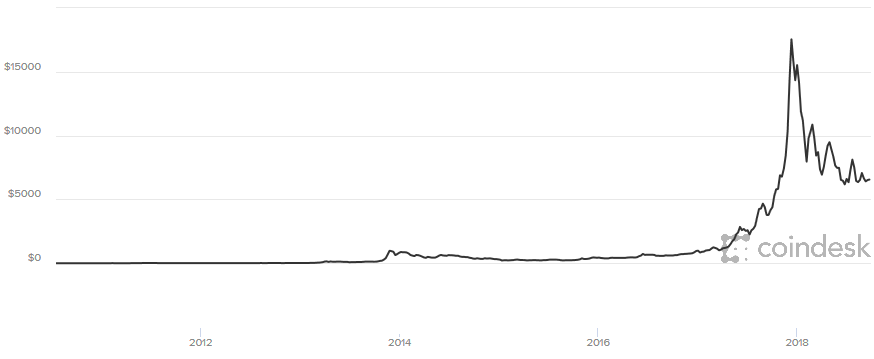
\includegraphics[scale=0.4]{\ImgPath/rys/bitcoin.png}
\end{center}
	\caption{Bitcoin price over years}
	\label{bitcoin}
\end{figure}

But financial prospects are not the aspects this thesis is concerned with. The most groundbreaking features the blockchain posses and which actually put it into the focus of modern computer science are anonymity and trustlessness.
\begin{itemize}
\item Anonymity: In the simplest implementations of blockchain such as bitcoin it is not possible to find any information of the user participating in the network. That is a simple consequence of relying purely on assymetric cryptography and no other requirement for allowing to interact with the network other than having a key pair. This simple feature has amazing implications in the real world. Every one in the world with internet connection can actually use blockchain. Coupled with the fact that cryptocurrencies can be used for value storage a way of escaping unstable national currencies has appeared for every human being. Recent example of that can be seen in Venezuela \cite{Venezuela}. There are also people who have found ways to use the anonymity in an illegal way. Silk road, the greatest illegal drug webshop accessible by TOR network has experienced a renaissance every since bitcoin payments have been implemented \cite{Silkroad}. 

\item Trustless: All of the currencies in our world are based on trust. The paper money has only a fraction of the value we assign to it. The numbers in our bank accounts have virtually no value. Currencies are simply are major agreement between all of the people on the world. In this world central parties are required such as banks which hold record of all transactions. We trust banks that when we ask them whether a person willing to buy from us has enough money, a true information will be sent to us. The double spending problem is solved this way. But blockchain has it's own mechanisms for this and thus allows us to omit the central party. We call the blockchain a trustless system because there is no trust required when interacting with other parties on the blockchain. Everything is taken care of by the computers, algorithms and protocols. The most grand example is Bitcoin itself which serves as a currency and a bank for all of the participants.
\end{itemize}

The element of blockchain technology that needs explanation is creation of a new block. As described earlier, in Bitcoin it is achieved by computing hashes of random numbers until a hash with certain amount of zeros at the beginning is reached. The whole process is commonly referred to as mining. This amount of zeros is called \textit{the difficulty}. The purpose of \textit{the difficulty} is to simply hold the rate of blocks being created constant. That is lower the difficulty when there are few miners and the transactions would be processed very slowly or increase the difficulty when everyone starts using supercomputers for mining. Currently, the rate is adjusted every 2016 mined blocks. More exact information about this topic can be found on bitcoin wiki \cite{Bitcoinwiki}. One important question that is left to be answered is: why do miners should bother with mining? Especially, why do people mine transactions which are not theirs? The answer is \textit{reward} and \textit{fees}. Currently, every mined block grants the miner who has done it some amount of bitcoin, that is a \textit{reward} for mining. Additionally, people simply willing to use Bitcoin for transaction purposes can attach fee to their transactions so that miners will be more likely to mine those transactions first and receive the fee. 

But looking for specific hashes is only one way of controlling block creation rate. PrimeCoin is especially worth noting as its method of mining is by finding prime numbers. Mining itself has also become a major part of computer hardware world due to computing power is has accumulated. Mining hashes is nowadays done only by GPUs due to parallelism benefits. There has been even created a special hardware called \textit{ASIC} which exist solely for the purpose of mining hashes.

After the subject of mining has been explained we encounter another problem. We know that after a block has been mined it has to be propagated throughout the network as to be actually accepted by the network.
What happens when in a large network two blocks are mined at the same time and both are able to propagate only through a part of the network before they collide? Then at least the majority of the miners ( that is 51\% of all computing power) has to decide which block to link to the blockchain and which to throw out. It is very important that a solid method of choosing the block by majority is used in a blockchain implementation because otherwise a malicious party could take over the network in some way or another by forcing his blocks with his transactions. It it also possible that the declined block will not be thrown away but will start living his own life in a sequence of events that are known as \textit{forks}. What follows is that one blockchain is split into two smaller ones which live from then on their own lives. Most of the time forks happen because a new version of the blockchain implementation is being deployed and not everyone wants this new version. This situation has occured with Bitcoin multiple times and the whole subject is worth thesis on its own.

\section{Ethereum}

Ethereum is one of many implementations of blockchain technology. It differs from the many other ones in that it is as a next step in the evolution of blockchain. Learning from Bitcoin mistakes and trying to create a flawless general-purpose blockchain implementation, Vitalik Buterin together with other programmers have published a paper outlying desing for Ethereum \cite{Ethereum}.  The new cryptocurrency has been officially released in year 2015. 

Owing to a plethora of new features, among which smart contracts are most notable, Ethereum has managed to become one of the most widely known and used cryptocurrencies in the world. It was the first to acquire support of real-world corporations. There are also actual companies serving products based on Ethereum. Being one of the cryptocurrencies it has also became a big part of the financial cryptoworld and has gone trough phases of big volatility, which can be seen on the graph \ref{ethereum}

\begin{figure}[!htbp]
	\begin{center}
\centering
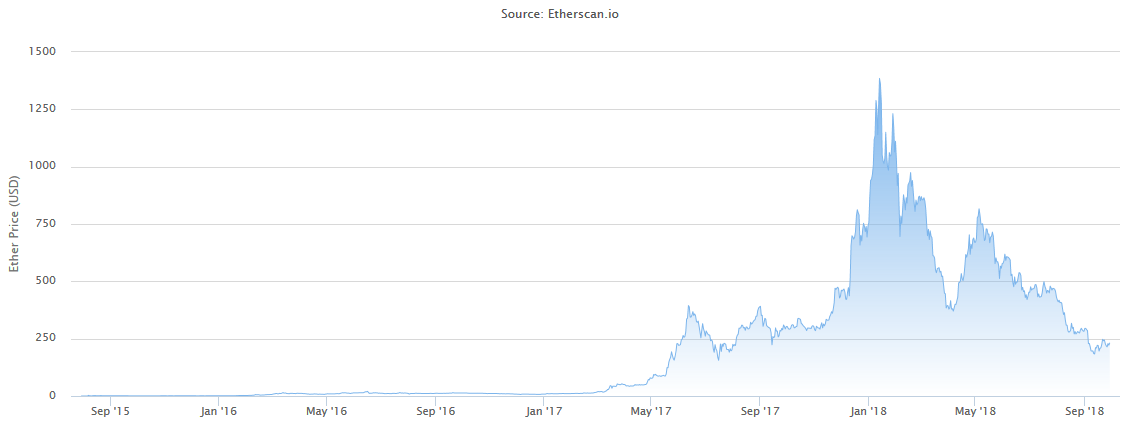
\includegraphics[scale=0.4]{\ImgPath/rys/ethereum.png}
\end{center}
	\caption{Ethereum price over years}
	\label{ethereum}
\end{figure}

The are a couple factors which make Ethereum unique and can be seen as an improvement over Bitcoin. 
\begin{itemize}
\item Faster and more scalable than Bitcoin: Every cryptocurrenct has scalability issues which stem from the fact that theoretically every network participant should posses the whole blockchain. But Ethereum team has gone one step ahead and started creating tweaks for this problem. While estimated peak performance of Bitcoin is that of seven transactions per second, Ethereum has managed to reach performance of twelve transactions per second. The most important fact tough is that constant research is being carried out which should find the solution for the scalability problem. So far the only discovered methods for solving this issue consist of sacrificing decentralization and thus security of the network.

\item Proof-of-Stake: As explained earlier, when two conflicting blocks meet on Bitcoin blockchain, the majority of miners have to decide which block to accept. This way of solving conflicts is called Proof-of-Work. The problem with this approach of using miners in general is that a lot of power is being used by the hardware around the world to power the different blockchains. The amount of power being used is apparently comparable to energy consumption of some smaller countries \cite{energy}.  Ethereum team is willing to change that by using Proof-of-Stake mechanism. This way the whole notion of mining is being eradicated. To create a new block a group of network participants is being asked to confirm transactions. The group has to be big enough so that the amount of coins they hold on specific blockchain sums up to 51\% of all the coins present on this blockchain. What follows is that only a fraction of the energy will be consumed and the network is still secure because a person willing to take over the network would have to buy 51\% of the coins on this blockchain. If we assume that market forces are working properly then the intruder probably will not have enough resources to carry out the attack. Nevertheless, it can be seen that we switch from one problem to another and users of Ethereum should be wary of that. 

\item Smart contracts: The single most important notion which differentiates Ethereum from all the other blockchain implementations is that of a smart contract. The general idea is that Ethereum blockchain has an Ethereum Virtual Machine(EVM) built into it. Which actually serves similar purpose as Java Virtual Machine for Java. If we put some lines of code of a language called Solidity into the transaction part of a block, the code will be executed after confirmation of this block. What smart contracts, EVM and solidity actually are will be explained in the next section. The most important fact is that thanks to this invention we are actually able to store not only static data in the blockchain but also code which will be executed. Thus, we acquire a fool-proof method of storing and carrying out procedures.
\end{itemize}

Immediate result of this invention are what's called Decentralized Applications(DAs) and Decentralized Autonomous Organizations(DAOs). If we call a typical blockchain a trustless database then we could call Ethereum blockchain coupled with solidity code a trustless application. Referring to a bank example mentioned earlier which can be replaced by blockchain for storing money but nothing more, we can see that now we are able to replace a banking entity also in such aspects as periodic payments or loans. Actually any operation which required intermediary can be now replaced by a piece of code which will be used by both side of the contract. The only requirement is that the deal has to use Ethereum and has to be carried out on the Etehereum platform. Fulfilment of those tasks can be achieved by construction of a Decentralized Application. 

If we go one step further we notice that is actually possible to create another cryptocurrency on top of Ethereum. Just as Ethereum is backed by a Proof-of-Work or a Proof-of-Stake we can create our own coins which will be backed by smart contracts, which in turn are backed by the Ethereum mechanisms. Those coins are most often called tokens. Finally, if a DA is created which facilitates it's own token we end up with a self living entity which trades its own money with it's own set of rules. That is what we call DAO.

As for the moment of writing this work there are almost two thousand DApps ( more popular naming of a DA ) serving purposes ranging from video games through social interactions up to financials \cite{dapps}.  Additionally, almost seven hundred tokens are being lively supported \cite{tokens}. 

Lastly, it is worthwhile to elaborate on the topic of cryptocurrency creation using smart contracts. The process goes by the name of Internal Coin Offering(ICO) which is taken straight from Initial Public Offering(IPO). IPO is simply what happens when company starts listing itself on the stock exchange. ICOs  pursue similar position as they mostly go hand in hand with a deployment of a fresh DAO. The coin offerings have become a vital part of the cryptocurrencies world as they have managed to earn millions of dollars and have become a new way for companies around the world to gain funding. Another sign of blockchain technology binding itself stronger to the world of real life usage.

\section{Smart contracts}

Smart contracts are files of code written in programming language called Solidity which are stored on blockchain and executed by Ethereum Virtual Machine(EVM). The specifications of the EVM will not be examined in this work as the material reaches outside of the aim of this thesis. Most of the information can found easily in the Ethereum yellow paper \cite{ethyellow}.  The notion of EVM will be touched upon in the last chapter where specific methods of code compilation will be described.

What needs explanation are the characteristics of Solidity language. It is an object-oriented, high-level language for implementing smart contracts. It's syntax has been influenced by C++, Python and JavaScript. Solidity is statically typed, supports inheritance, libraries and complex user-defined types among other features. Additionally, it is turing complete. It is very important to notice that blockchain serves overall a similar function to that of a database. But databases in general offer us SQL or SQL-like languages which are not turing complete without considerable extensions. Solidity in turn offers us a different perspective. We are able to experience a language which deals with directly with data storage but offers us the possibility to solve most computational problems at the same time. Of course SQL languages are declarative and operate on different types of data structures thus serve other purposes. But we can see that a new frontier has opened in the data storage world.

It is also important to understand the implications of programs running on blockchain. As every transaction done on blockchain has to be stored on blockchain it is also true that programs running on blockchain have to save their every change of the state on the blockchain. Thus the actions have to be confirmed by other users of the network and propagated. It is now possible to create program by a malicious user or by a bug which would spam the whole network and thus make it unusable. For example, an infinite loop in a smart contract would need constant confirmations and would not allow others to do anything with the network. To circumnavigate this problem a notion of \textit{gas} is introduced. Every smart contract put on the blockchain has to have some amount of Ether assigned to it. Every line of code run on this contract consumes gas. Different operations cost different amount of gas. For example, read operations cost no gas but sending ether from contract to somewhere else costs a lot of gas. The gas amounts can be found easily on the internet \cite{gas}.  The amount of gas respective operations consume is fixed. But the price of every gas unit denominated in Ether is subject to change. To run a line of code the contract has to pay product of amount of gas used and current gas price. The gas price is shaped by many factors but it is mostly set by miners. As a result the infinite loops would eventually run out of funds to consume and would stop. Moreover, usage of gas and not simply Ether lets those two values be decoupled. Thus a double increase of Ether value will not directly affect the gas price. Still, the gas price can change and thus we can see that big smart contracts are discouraged as they can become expensive to use. 

Just by this fact we can see that programming in Solidity is specific and requires careful considerations in many areas. Most notably those areas would be:
\begin{itemize}
\item Gas optimization: Besides cost of running code there also come costs of storing data. Because every variable or data structure used in a smart contract also comes with a cost. As a result we could notice a similarity to the old days of programming when computing power and more importantly storage space were scarce. A Solidity programmer also has to use a lot of tricks to keep his code small and fast. Unfortunately, the history of software development has shown that such practices often end up in a code that looks badly and is unmaintainable. Remedy for possible future catastrophes could be usage of open-source libraries which hold optimal fault-proof solutions, future developments in language which would abstract the gas optimization away and extensive testing.
\item Security: Ethereum is all about money and the end purpose of Solidity is automation of money handling processes. An immediate consequence of those facts is that Ethereum world is a breeding ground of malicious users which will use every possible loop-hole in the system to steal the biggest possible amount of funds possible and then perish behind the veil of anonymity. The problem with stealing on blockchain is that once it is done it is done. If we are not able to connect the public address of the hacker with his real world identity then there is nothing we can really do. Moreover, the gas optimization practices stimulate creation of unsecure code. Fortunately, the issue has been noticed by the community and there are plenty of materials allowing for education in those matters. The documentation of Solidity being a good starting point \cite{secure}. 
\item Bugs: Solidity is one of the most costly language in the world when it comes to bugs. One bad mathematical operation could create a completely wrong address of transaction receiver and thus result in a transfer of millions of dollars to a dead account. It has happened before and is still happening. Testing is one of the most vital aspects of Solidity programming and an aim of 200\% test coverage should not be treated as a joke. It is also a good practice to use private test blockchain networks where funds can be created out of thin air. Those networks can be used for integration testing and such. Ethereum itself offers three world-wide networks besides the main one which only purpose is letting user test their contracts and letting Ethereum developers test new solutions. These networks are named Ropsten, RinkeBy and Kovan. 
\end{itemize}

It is obligatory for the language to allow for a communication with an outside world. That is to allow for external parties to read the blockchain data and interact with the blockchain state. The task is achieved by a Remote Procedure Call(RPC) communication as well as by Inter Process Communication(IPC). In this work the RPC variant is being used and explained due to it's versatility. The messages used are simply JSONs. The whole API reference can be found on ethereum wiki \cite{RPC}.  Our client has to connect to an Ethereum node which serves and appropriate end-point through HTTP. As the API is quite simple a ready implementation of the communicator can be found in most of the widely used programming languages. The general standard of RPC messaging used by Ethereum goes by the name web3. As this project used Java, the library web3j was used. Still, web3.js for JavaScript or web3.py for Python could have been used as well.

%-----------------
% Current state of the technology
%-----------------
\chapter{Current state of the technology}

In this project blockchain will be used to enable decentralized and trustless loan servicing. The idea of transferring this major business into the crypto world has quickly become one of the first use cases of the technology. As such, it is possible to observe a multitude of solutions present on the market. Each coming with it's own innovative mechanisms, it's own strengths and it's own weaknesses. Generally, there are two main points differentiating approaches to this problem. 

Firstly, it is noticeable that most of the loan service providers specialise in one certain branch of the loan business and offer services in only this branch. For example, there are companies offering just normal loans to people in need of money whereas the cash to lend is provided by people willing to invest their money. Some other companies organizations focus only on letting you leverage your trading by usage of loans. Finally, there are some cases of business offering possibility to automate real life loan processes using blockchain.     

Secondly, everyone has it's own approach to dealing with the problem of lack of loan repayments. When a person lends money to someone he immediately wages a risk that the borrower could go default and could stop repaying his loan. Leaving the lender with nothing. Situation especially dire in the world of blockchain where it is not so easy to reclaim your money on your own. Fortunately, some remedies to this problem have been found and are widely used. The example being, backing your loans with collaterals or sharing your personal data for the sake of possible legal procedures.

In this chapter some of the most prominent products or systems will be presented and grouped according to the two points mentioned above.

\section{Normal loans}
The first group concerns typical loans. The kind that first comes to our mind when somebody hears the world \textit{loan}. The only difference here is that the entity providing loans is not some company but other people.  In this business model the companies provide the technology for matching the borrowers and lenders or help lenders have their money back. For this they receive minor fees. All of the processes related to granting loans or setting interest rates are automated and controlled by the market forces.
One could ask, what is the difference between those firms and the ones not using blockchain for this type of loan providing? The answer is that if the cryptocompany resorts to a minimal usage of cryptocurrencies it will still automate the loan contract itself. Therefore, no legal documents are really required as all of the essential financial procedures are saved on the blockchain. Traditional company will always have to create some legally binding document which in the essence will be based on trust between borrowers and lenders.

Beginning, a company named \textit{ETHLend} \cite{ethlend} is examined. Created at the brink of the year 2017 ETHLend has, so far, successfully implemented the idea described above. The whole system is based on Ethereum and allows for deals using Ethereum or tokens based on it. Users create their anonymous accounts to which credit history is slowly accumulated with progression of time and repaid loans. The loans require a collateral which will amount to some part of the loan. The collateral is most often some other cryptocurrency. We can see that in the essence, the company simply allows us to leverage our holding by exchanging the currency at the same time. Additionally, an ICO of a coin named \textit{LEND} has been carried out at the inauguration of the company. The funds gained during the ICO have been used to cover expenses of the company and invest for future development. Moreover, the LEND token can be also used for lending and allows for some extra functionalities of the system. ETHLend is an interesting example of blockchain company successfully using the technology to fill business needs and properly finance itself.

Going forward we approach next big player on the market. It is named \textit{BTCPOP} and here the customer can take part in normal loan business \cite{btcpop}. But the whole site is a much more developed system. Being created in the year 2014 it had the chance to extend it's line of business with a good dose of diverse features. Foremost, BTCPOP puts special focus on business to business contracts. We can invest in specific companies with funding their loans requiring much bigger capital and thus needing additional safety mechanisms. Besides, the already present on the market collaterals of the loans and supply of personal information for legal purposes the investors are also secured by insurance contracts which are maintained by the company itself. Moreover, one can publish bonds or create your own IPOs making it possible to for companies of all sizes and all funding needs to discover their need being fulfiled by BTCPOP. Every investor has the possibility to put his funds into a mining pool. Those money are being used to buy hashpower, that is simply usage time of a big rack of GPUs, and mine the specific kind of cryptocurrencies an investor chooses. Lastly, the company provides normal exchange services allowing to trade cryptocurrencies. 

Next on the list stands \textit{Bitbond} \cite{bitbond}. Being very similar to the previous firms it focuses mostly on loans on a peer to peer basis. This time the focus it put mainly on the loan business and nothing else. Bitbond puts above average effort into the registration procedure for new user going as far as requiring video confirmation of your persona. Additionally, a special feature for investors is offered here. Fund granters can ask the system provided by Bitbond to automatically manage their fund and allocate them in the loans most resembling their risk propensity, durations and many others. This type of automatic asset management is so far endemic to this company. One can see how minor technological innovations can put blockchain based companies into advantageous position on the market bringing making investing in loans easier and more accessible. Of course, the intelligent investing machine comes at additional fees.

The last company mentioned on the list of typical loan providers based on blockchain will be \textit{Credible Friends} \cite{credible}. The market put under investigation here is that of credit cards, daily shopping and close friends networks. Usage of the application looks as follows. We invite our friends, that is people we actually know and trust, into our network. We assign every one of them a threshold of credit value they can loan from us. Now, whenever one of our friends goes to but some clothes, for example, he uses the application as a credit card, where the money come from us lending them.   The interest rate is fixed to 25\% APR( equivalent of polish RRSO ). The mission of Credible Friends is simply make the credit card market decentralized and freeing consumers from the need to use banks. We can clearly, see that just another brilliant way of filling market hole just by using new technology. Though, the problems credible friends encounters and will encounter in the future will be always entangled with lack of scalability of most blockchain implementations and related slowness of transactions processing.

\section{Cash for coins}

The whole cryptocurrency market has experienced waves of tremendous volatility at least a couple times. For a couple of years already, the market movements have created a general market opinion that blockchain technology is a diamond yet to be uncovered and thus made everyone await appreciation of their holdings in cryptocurrencies. Masses of new investors have succeeded in a scenario of a typical self-fulfilling prophecy and made all of the prices really go up. Making everyone ignore, the massive security incidents, intricate flaws of the blockchain itself and many other technological aspects. As a result cryptocurrencies have lost their status of utility products which would simply start being used instead of normal currencies like dollars or polish złotys. Instead they became stores of value. That is, it was more  clever to simply hold the coins, wait till they increase in value and then sell them rather than normally use them. 

Suddenly, a new market opportunity has appeared. Some clients wanted to still hold their crypto assets but were in need of cash which they would actually spend. As a result a new branch of loan business has risen up. Companies that take your cryptocurrencies as collateral and transfer some part of the collateral value as cash to your account. The moment you give the cash back with some interest sprinkled in you receive you cryptocoins back. By that time you expect that the value of crypto assets has risen enough to cover interest expenses. If it has fallen you lose twice. Firstly, on the asset depreciation. Secondly, on loan interest. Following are presented some of the companies delivering this exact service.

The first position on the list is \textit{Kambo} \cite{kambo}. Created in year 2010 it is one of the oldest companies dealing with blockchain on the world. Proving a point that entrepreneurial spirit using even such a new and undiscovered technology can withstand the test of time. What's more, Kambo is employing over one thousand workers in almost twenty countries. Being at the same time one the biggest cryptocompanies. The business model of Kambo is exactly what has been described earlier. Person in need of dollars can park his crypto assets on Kambo account and receive 50\% of the value he left on his real-life bank account. The moment he pays the money back plus interest he gets his crypto back. Kambo can be a great of example of a mature usage of blockchain technology and the stable profits it can make. So far though, it does not provide any special traits which would differentiate it from it's rivals. Putting it at risk of losing market strength due to lack off innovative actions.

The next pretender to market leader position is named \textit{Unchained Capital} \cite{unchained}. Just as for Kambo it's focus is on granting people USD for BTC while holding their BTC in a partial ownership. The strategy of Unchained Capital for gaining an important role on the market is exactly what makes the whole crypto market so rapidly changing and innovative. They put great focus on making their collateral holding as safe as possible by explicitly stating that every user has it's own address which could be compared to creating a new account for every user in a bank. Solution widely used in real-life banking but not so widely used in crypto due to increase in maintenance costs. Additionally, Unchained Capital does not rely on your personal information to confirm your credibility but rather use special algorithms for analysing your blockchain addresses to check if your loans will be repaid. The feature is rather experimental but that is why it's tried by a start-up like company.

The last case on the list is that of a failure. It is worthwhile to look at examples of what follows from a badly designed business model backed by an unimpressive software. The company goes by name \textit{Salt Lending} \cite{saltlending}. It has been abandoned not long ago by it's CEO and is currently on it's way towards bottom. Salt Lending was a very interesting company for clients because it allowed to receive as much as ten times the value of stored crypto in USD. It is especially impressive when we consider that it is actually a loan of 1000\% value of the collateral compared to 50\% offered by Kambo. But Salt Lending id not offer any special safety measures or some amazing machine learning algorithms for determining it's debtors credibility. The whole business has quickly became unsustainable and started being abused by clients taking immense loans and running away. One should learn that from this example that offering extraordinary business offer with ordinary technology backing it will not end well.

\section{Leverage}
So far two possible loans have been discussed. The first called normal loans which are seen by receiver as receiving something for nothing backed eventually by collateral. While the currencies are mostly the same.  Seconded by loans allowing to exchange crypto for real-life cash. The next type of a loan that will be discussed is the one happening when cryptocurrencies are exchanged for cryptocurrencies. This type of transaction is mostly called leveraging and is widely used in the normal financial world. What is leveraging for? The most used application of leverage is that of trading stocks. Lets assume we have an X amount of cash. We expect that certain stock price is obliged to rise and thus are willing to invest a lot of money to earn on it. Being so sure of the price change we decide to take up a loan so big that we end with cash amount equal to 10X. What happen if we invest either sum and the price moves upwards by 10\%? Investing X would result in a profit of 0,1X. Investing 10X would earn us whole X minus the interest of the loan. So long the interest is low enough we are able to earn much more just by having certainty in the stock price movement.

An interesting though experiment could follow if we imagine that by some clever research we discover that some market movement will happen with a probability of 100\%. Now lets say the price change is denoted by Y. No matter what size Y is we could always leverage ourself so much that as a result we would earn millions of millions of dollars. So long we are able to get the interest rate lower than the relative price movement we are able to change one thousand USD into a sum big enough to cover all imaginable life expenses. All of that would happen only because we had the certainty thanks to information. That is a reason a finance person would say we live in an information era.

Of course cryptocurrencies could not leave such a lucrative area of the financial world aside and a multitude of different companies serving leverage services has appeared. Below is presented the most interesting case the other ones are left untouched as they mostly use the same techniques as in normal loans. One key concept that has to be introduced here is that of a \textit{stablecoin}. As proven already multiple times in this paper cryptocurrencies are very volatile. The problem that ensues is that such instability of currencies results in an instability of companies and deals basing on those currencies. Solution invented for that problem is exactly what one would call a stablecoin. That is, a coin whose value is fixed at some certain value. Currently, the title of the most widely used stablecoin is held by \textit{Tether}, where value of one Tether is fixed at 1 dollar. The fixed ratio is achieved by restricting the possibility of mining new Tethers to central party and holding exact sum of USD on the central party's real-life bank account. One can see that Tether simply exchanges the decentralization aspect of blockchain for the stability. An action deemed nonsensical by many as the whole idea of trustlessness completely evaporates.

\textit{Maker} is company which created a cryptocurrency called \textit{DAI} \cite{makerdao} and this cryptocoin is also a stablecoin. The difference between DAI and Tether is that DAI is not centralized in any way. To explain how stability is achieved here one has to look at the general loan granting process. To borrow a loan using DAI you have to deposit some Ethereum in a special smart contract called collateralized debt position(CDP). Then you are able to withdraw DAI from CDP. The value of DAI withdrawn has to be smaller than the value of Ether you have stored. This process is called over-collateralization. Thanks to this process your DAI is always pegged to an equivalent of 1 Ethereum because you simply switch your Ethereum to DAI using smart contract. If Ethereum price changes the possible amount of DAI you can withdraw from CDP will also change. Finally, when your Ether stored on CDP will not be enough to cover the currently possessed DAI the contract gets liquidated. Your DAI and CDP are destroyed and the Ether comes back to you decreased by a liquidation fee ( most times 13\% ). On the other hand if everything goes right you give back the DAI plus interest later and can take your Ether back. One may ask now, what for should I use this scheme if as a result I will just receive different currency of which value will be lower than my deposit? To answer this question we go one step further. Lets assume we have taken the loan and exchanged Ether for DAI. Now we take the DAI to some exchange and buy Ether for it. We use this Ether to increase our over-collateralization and take more DAI. We can repeat the process and every time we will be able to increase the Ether collateral by a fraction of previous increase. The process will finally stop because the fraction will be miniscule. But in the end we may end up with twice as much Ether stored on our CDP than what we have started with. Now if the price of Ether increases we revert the whole process but this time we can buy the DAI for a better price than we sell it. Finally, our Ethere is more valuable and we have more Ether. But if the price falls down then we could end up liquidated and lose on value and on quantity of Ether. The whole financial process is reminiscent of rehypothecation used in the real-life financial world by banks to leverage and which has been one of many reasons for the financial crisis of 2008 to happen. The difference now is that DAI is on blockchain and follows the rules of publication of every transaction thus every action can be traced and reacted upon. In the year 2008 must of the contracts and deals were totally obfuscated and made the investors commit uninformed transactions. DAI could be treated as one of pearls of the blockchain technology, granting stability but leaving the decentralization and trustlessness aspect untouched. Of course, there is much doubt whether the whole project will take off. Following the process described above is even harder than understanding it and thus horrid user experience could a nail to the grave for the project. Moreover, the idea being quite fresh it is still doubted whether everything is secure and if it just a matter of time for the malicious agents to find a loophole in the system and put it to ruin. The only safe choice right now is to wait.

\section{Loan automation}

The last position on our list of major blockchain projects impacting the financial loan world will touch upon corporate solutions. All of the aforementioned chapters focused on companies whose business model resembles Software as a Service (SAAS). That is the loan company is a separate entity that simply provides some kind of GUI or API through which we can interact with the loan service. An area not explored yet is one that would resemble Infrastructure as a Service (IAAS). In this case, the blockchain company would partly integrate their services with processes of client's company. For example, a bank could ask to transform their retail loan processing into one using blockchain but at the same time it should still integrate with other systems such as bookkeeping, trading or risk quantification. We can see that what is needed here is not simply API or GUI but a whole solution tailored to this specific firm's needs.

The blockchain market has not evolved yet to hold many companies which could provide services of such magnitude. Nevertheless, we can see some companies basing their first footholds in this domain. One of such companies is \textit{Othera} \cite{othera}.  Being mostly still in development there is not much news coverage on it and being focused on corporate clients it is hard to acquire any informations on test usages. The general idea though is to create two big platforms, one which would focus on loan business and a second which would allow for exchange of cryptocurrencies and tokens. The systems would integrate with clients in an appropriate way to their business and let everyone partake in the trades. Benefits stemming from this integration would be an increase in liquidity thanks to new loan markets and new routes for the flow of capital. Othera itself would earn on fees and contracts for integrating new clients into the system. As good as the whole idea sounds there is still little to be said about the reality given that Othera is first of it's kind and still has not properly started. It would be wise to observe the future developments and occasionally check if this specific branch of the market is gaining momentum.

%-----------------
% Software design
%-----------------
\chapter{Software design}

Not every system has to be designed before being implemented. Especially if it's destiny it to never be used by anyone outside the creator or if the aim of the system is to make life of everyone using and supporting it as painful as possible. The system created for the purpose of this thesis does not fulfil either one of those requirements and thus a specification and an architectural design had been created before the construction  began.

\section{Loans} \label{loans}
One loan offer on an exchange will consist of following parameters, which will be specified by the user before every deal:
\begin{itemize}
\item \textbf{Basis}: Size of the loan denominated in Ethereum.
\item \textbf{Duration}: The time after which the whole loan should be paid back together with interest. Depicted per predefined amount of days.
\item \textbf{Interest}: Percentage of the loan basis which has to be additionally paid by loan taker. Calculated per predefined amount of days.
\item \textbf{Collateral}: Information whether the loan is backed by a third party and has a low probability of going default. For example loan taker with no evidence to back his repayment probability will have only access to loans with collateral parameter being equal to None. At the same time loan taker with his loan being backed by a special bank agreement will have access to loans with collateral being equal to Yes. The deposit granted by bank agreement will have an amount equal to the loan basis plus interest incurred. Additionally, the deposit will be a smart contract connected to the loan smart contract.
\item \textbf{Collateral address}: If some kind of collateral will be specified an accompanying address of a smart contract serving the purpose of this address has to be specified. 
\end{itemize}

Besides the user specified arguments the loan will be also customized according to the properties held in a properties file held inside the system. The arguments are:
\begin{itemize}
\item \textbf{Scale}: Due to properties of Soliditiy language which are described in the chapter \ref{solidity} all of computations done in system will be done using integers. That means values of decimal representations have to be scaled up so that they become integers. The scale factor is used across the program to maintain correctness of computations done.
\item \textbf{Precision}: Also coming from Solidity peculiarities the exponential function will be calculated using Binomial Expansion. \textit{Precision} is an additional variable that exactly determines the number of iterations of for loop calculating the approximation.
\item \textbf{Payment Period}: Used by duration processing to determine if enough time has passed for the next repayments to be processed. The value has to be given in miliseconds as the time on blockchain is represented in UNIX format.
\end{itemize}

The process of buying and selling loans will have the same characteristics as the one seen on the stock exchange. That is loan ask whose size exceeds size of one respective loan bid will automatically cover the second identical loan bid. For example loan taker A asks for a loan of 1 ETH. There are two identical offers by loan provider B and C both equal to 0.5 ETH. The matching will automatically buy for A both loans from B and C. Moreover, if loan taker asks for a loan of interest higher than the lowest present on the market he will be sold the loan with the lowest interest. For example loan taker asks for a loan of interest 2\%. There are loans on the market being bid with both interest of 2\% and 1\%. The loan of 1\% will be sold to the loan taker. In terms of repayments the loan will function as an amortized loans. That is, the repayments will be constant with principal amount being paid back increasing and the interest amount decreasing. The formula for computing the installments looks as follows:
\[C = \frac{rP}{1 - \frac{1}{(1+r)^n}}\]
Where C is monthly installment, r is interest rate per month, P is principal amount/basis and n is a duration of a loan in periods equal to predefined amount of days.

\section{Types of users} \label{users}

The project provides for three types of possible actors. 

\textbf{Loan providers}: Any user with spare Ethereum and access to the application. Such person bids his loan offer with specific parameters. At the same time the funds are transfered to the smart contract create by bid offer. After the creation of bid the loan giver queries the matching engine to look for any matches to the offers being present. If it some are found he confirms the creation of transactions and the loan smart contracts are created. Finally he can query the loan every repayment period for the repayments made by loan taker to be transferred to loan giver's account. If a query is sent and the funds are not sufficent for the predetermined repayment than the loan is blocked and collateral procedures step in. Those are described in section \ref{processes}.

Why are the funds sent already during bid creation and not creation of actual laon? It would not be possible to transfer funds later when the loan is created without explicit consent of loan giver. For the consent to be passed the loan giver would have to sign the transaction with his private key and as a consequence he could block the whole transaction until he does it. In the end, it has been decided that the cost of freezing funds inside loan bid is lower than the cost of blocked transactions. After all the loan bid can be freely cancelled.

\textbf{Loan takers}: User who lacks funds at the moment and is willing to sign a contract granting him those funds and obligating him to repay them increased by interest at later time. Loan taker creates loan ask in which it is specified what type of loan he is willing to take upon himself. Having little to no funds he is only obliged to pay for the transaction cost of creating loan ask. Loan taker has the possibility to specify collateral type he is willing to grant. In return he can expect lower interest rates accordingly to the risk level he assure of. If some kind of collateral is specified he also has to specify address of a smart contract fulfilling role of this collateral. There are possible collateral options:
\begin{enumerate}
\item None: Meaning the loan taker grants no assurance that loan giver will receive any kind of his value back in case of default.
\item Deposit: That is usage of a collateral deposit from a third party. The deposit has to cover the whole value of loan, that is principal plus all of accrued interest. Example of such real life case using this option is following. Close friend of a loan taker has enough funds to grant him the loan but is not willing to waste time on care for the whole loan repayment process. He is willing to create a back up deposit because that will cost him no time. He can later withdraw the fund if the loan is successfully repaid. If the unfortunate happens and the deposit it granted to the loan giver then the deposit maker can pursue the loan taker as he knows him personally. 
\item Legal informations: The middle option in respect to risk is granting the loan giver a possibility to pursue legal procedures after the loan goes default. For this to happen a designed procedure happens. The loan taker goes to a notary and asks him to create a smart contract containing his personal information. The notary encrypts the information with some key designed for encrypting big chunks of data and then uses his public key to encrypt the data key. Both the encrypted data and encrypted data key are stored in smart contract described as smart contract for legal procedures. The data has to be encrypted because it's publicly accessible on the blockchain. If loan goes to default a flag is set on the smart contract for legal procedures. The notary can then grant the loan giver the private key to decrypt data key, which in turn will be used to decrypt the data. The data will be used to follow legal procedures by bailiff of a country where the loan taker is located.
\end{enumerate}

\textbf{Authorities}: Third parties which create the collateral smart contracts used by loan taker. In the case of deposit it will be a person having enough funds to cover whole loan expenses. He will create the deposit smart contract, transfer fund to it and grant the address of this smart contract to loan taker. The deposit maker can also withdraw his funds if the deposit is not being used. It is expected that the deposit maker will take the risk of backing loan taker because he has the ability to reclaim the money which are present outside of blockchain.

The second scenario uses notary who confirms the legal informations of a loan taker and encrypts it. He then creates a smart contract for legal procedures containing all of the required data except for his private key. This scenario includes also bailiffs which chase the loan taker after having received the required information. It is worth mentioning of the flaws this scenario possesses. For example, it is required that the API for creating smart contract for legal procedures is held only by the notaries and that those notaries will not let the access escape. Otherwise, anyone could create their own smart contracts for legal procedures and put anything inside it. The second problem that could happen is legal jurisdiction of the loan taker. It could so happen that there are no bailiff services there. Overall, the legal scenario requires that there exists a general trust in the third parties and breaks the trustlessness aspect of blockchain from this side.


\section{Processes} \label{processes}

It is required that all of the processes composing the whole system will be carefully planned. This way any sort of high level misconfigurations can be pointed out and fixed. The processes in this work are presented using BPMN and are accompanied by short notes explaining more intricate concepts.

\begin{figure}[!htbp]
	\begin{center}
\centering
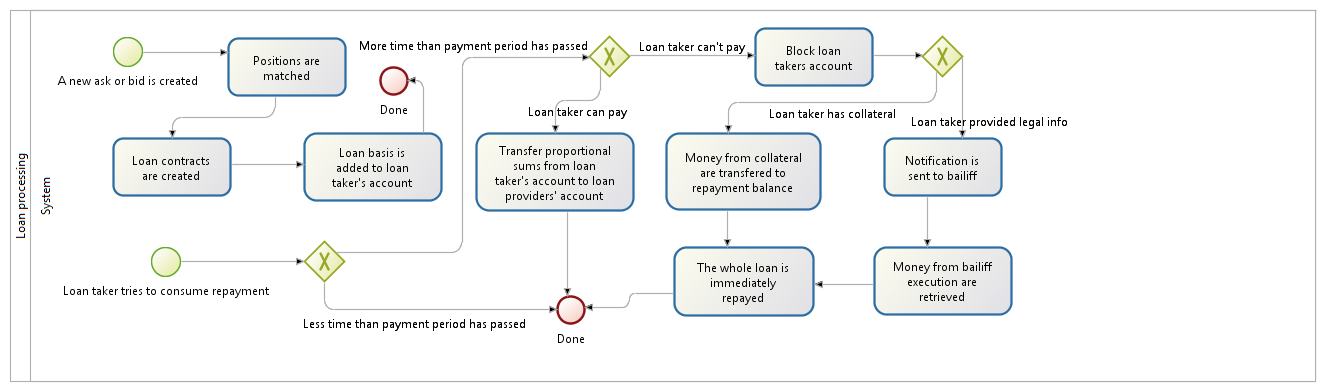
\includegraphics[scale=0.4]{\ImgPath/rys/loan_processing.png}
\end{center}
	\caption{Loan processing}
	\label{loan processing}
\end{figure}

The figure \ref{loan processing} gives us a glance over the whole life cycle of a loan. Starting with creation trough match of equivalent asks and bids, followed by regular transfer of funds and ended with eventual handling of going default. The loan is blocked as to not allow any possibility of loan giver draining the collateral funds from the deposit repeatedly. Only the sum left to be repaid should be granted to the loan giver.

\begin{figure}[!htbp]
	\begin{center}
\centering
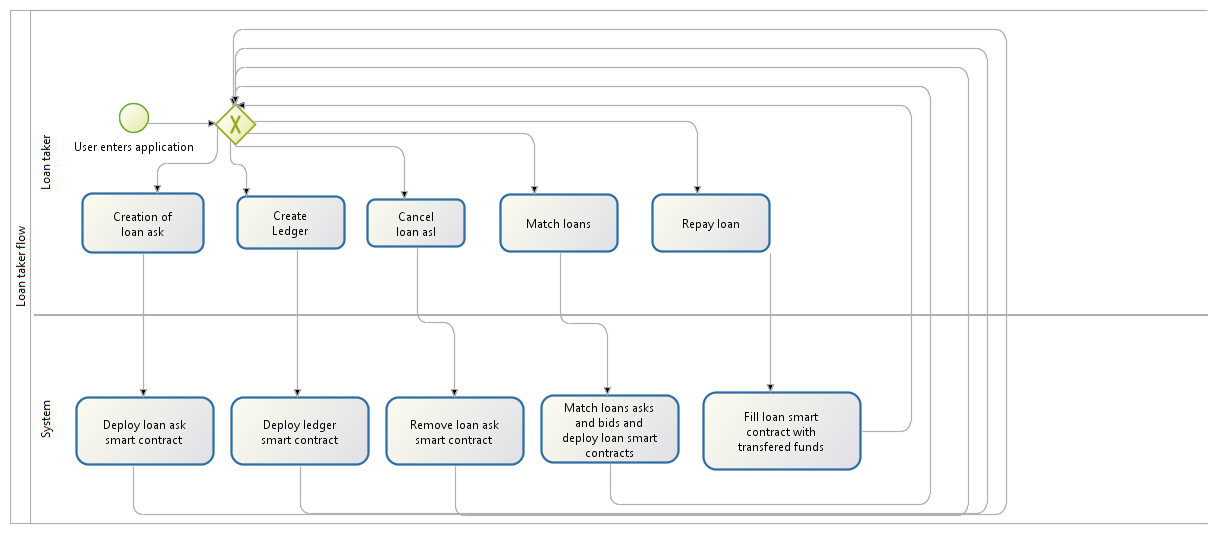
\includegraphics[scale=0.4]{\ImgPath/rys/loan_taker.png}
\end{center}
	\caption{Loan taker flow}
	\label{loan taker}
\end{figure}

\newpage

The figure \ref{loan taker} describes what type of actions will loan taker take during his participation in the loan processing process. At all times he is able to create new loan asks, cancel them, create new loans by querying the system to match the loan offers he can also repay the loans as he is supposed to do. New concept introduced here is that of a ledger. This entity will be described more thoroughly in the chapter \ref{architecture}. To give a quick explanation. Ledger is a point of storage of loan bids and asks. Every one can create their own ledger and give the ledger address to other users. Only loan offers on the same ledger can match.

\begin{figure}[!htbp]
	\begin{center}
\centering
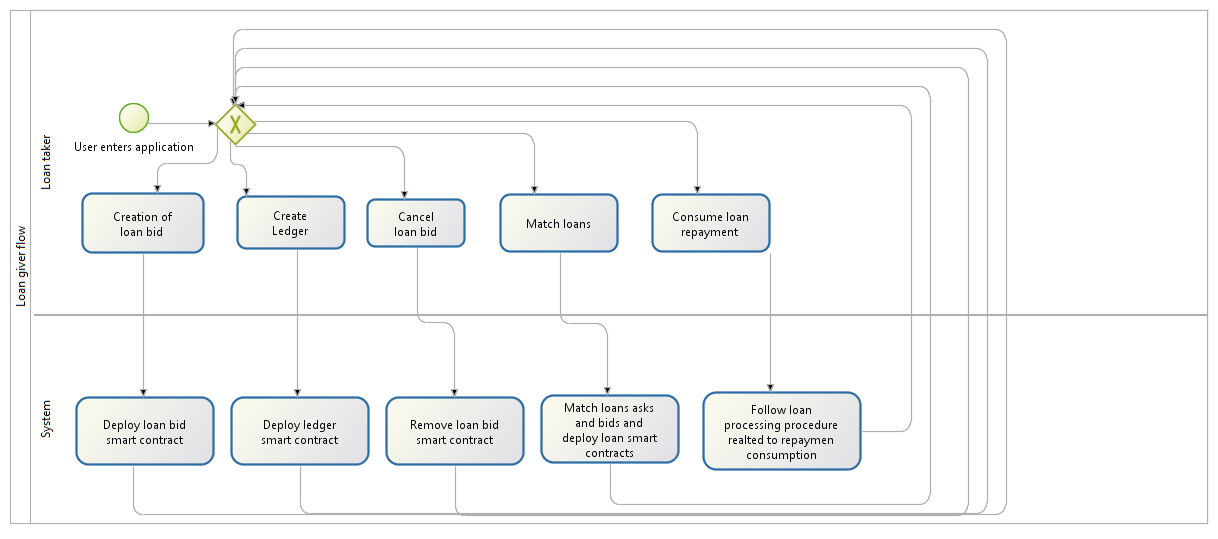
\includegraphics[scale=0.4]{\ImgPath/rys/loan_giver.png}
\end{center}
	\caption{Loan giver flow}
	\label{loan giver}
\end{figure}

Just as for the loan taker the figure \ref{loan giver} describes what type of actions will be taken during the loan processing process. The only noticeable difference here is that the loan giver is not given a chance to repay loans instead he has the possibility to consume the repayments and eventually call for help in case of defaults.

The last figure that is \ref{authority} explains to us what are steps one of the authorities stated as the collateral by loan taker will have to take. The steps have been already described precisely in the description of the authority users \ref{users}.


\begin{figure}[!htbp]
	\begin{center}
\centering
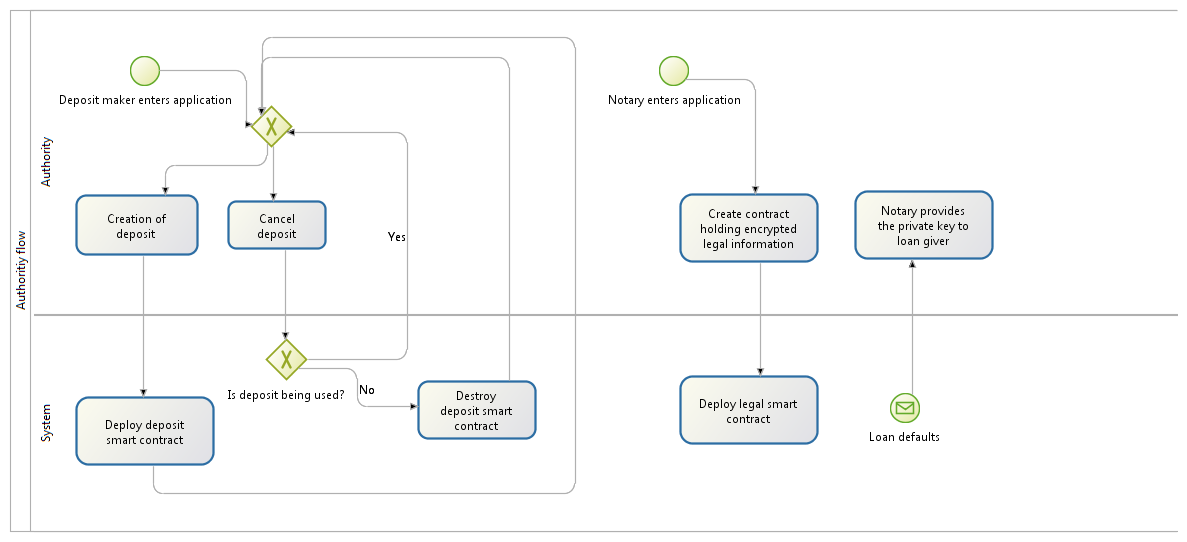
\includegraphics[scale=0.4]{\ImgPath/rys/authority.png}
\end{center}
	\caption{Authority flow}
	\label{authority}
\end{figure}

\newpage

\section{Requirements}

Having modelled the core components of the system that is key data structure (loan), actors in the system (users) and processes that will control the changes of state in the system it is possible to state all of the requirements the system has to fulfil.

The complete system should provide following functions:
\begin{enumerate}

\item Loan givers and loan takers should be able to:
\begin{itemize}
\item Create respectively loan bids and loan asks. Moreover, they should be able to specify directly the following parameters in their loan bids and asks: Basis, Duration, Interest, Collateral Type. Loan takers should be also able to add address of a collateral smart contract accordingly to the collateral type they have chosen.
\item Specify the indirectly the parameters: Scale,Precision and Payment period. Indirectly in this case means that the parameters are not stated through API or GUI but through properties file attached to the code. It is important to state that security of this aspect is consciously omitted. As it is not foreseen for the project to be deployed in a production environment there are no checks whether matched loan asks and bids have those three parameters equal. The reason being those checks are deployment dependant and do not fall into the area of concern this work deals with.
\item Create ledgers and share ledger addresses to other users.
\item Cancel all of their open bids and asks.
\item Check their open bids and asks as well as the whole public exchange.
\item Query the ledger of open asks and bids and use matching engine to create new loans.
\end{itemize}

\item Loan takers should be additionally able to:
\begin{itemize}
\item Transfer repayments to the loan contract.
\item Attach to their loan ask a smart contract containing their personal information encrypted by notary. The whole data should decryptable upon receiving notary's private key used for encryption. The smart contract is denoted as legal procedures smart contract or legal. The notary should grant the private key upon noticing the set flag in the smart contract. The setting of the flag should be done automatically and rely on no trust.
\item Attach to their loan ask a smart contract containing sum of funds sufficient to cover the whole loan cost that is principal plus interest. The transfer of funds from deposit to loan giver should be done automatically and rely on no trust.
\end{itemize}

\item Loan givers should be additionally able to:
\begin{itemize}
\item Consume repayments from the loan contract.
\end{itemize}

\item Deposit makers should be able to:
\begin{itemize}
\item Create a deposit with a specified sum of money.
\item Withdraw all the funds from deposit if it not being used.
\end{itemize}

\item Notaries should be able to:
\begin{itemize}
\item Create a legal smart contract with encrypted data.
\item Check the flag of a legal smart contract.
\end{itemize}

\item Every user should be able to:
\begin{itemize}
\item Access the application having only internet connection. That is no registration or background check is required.
\item Maintain his anonymity while using the system. Exceptionally, it could happen if loan taker has added legal collateral and went default.
\end{itemize}
\end{enumerate}

All of the other aspects mentioned in the preceding chapters are treated as external to the system and will not be included in the design. Those are for example, bailiff chasing the loan takers or decrypting the legal smart contract information.

\section{Architecture} \label{architecture}

The last step in the design process is creation of an outlay of the components which constitute the whole system and at the same time fulfil all of the stated requirements. The application created in this project  follows the Model-View-Controller architectural pattern and the respective components can be seen on the figure \ref{system components}. Through usage of REST and RPC a separation of the components has been achieved and thus every box in the diagram could be replace by another technology so far it complies to the interfaces.

\begin{figure}[!htbp]
	\begin{center}
\centering
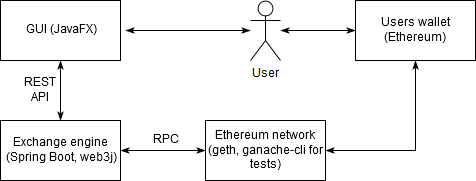
\includegraphics[scale=0.4]{\ImgPath/rys/high_level.png}
\end{center}
	\caption{System components}
	\label{system components}
\end{figure}

The respective components denote:

\textbf{GUI}: The View component is implemented as a desktop application. Standard Java library, JavaFX, is chosen. The choice is based on the wide usage of the library and easily findable support. The design of the GUI tries to follow the Material Design rules \cite{material} and uses another library based on JavaFX which provides the CSS styles and JavaFX components based on this design style. The supporting library is called JFoenix. The GUI module communicates with the Exchange engine using REST.

\textbf{Exchange engine}: The Controller component being a REST server uses Spring Boot at it's core. The framework lets us easily create a running REST server and add new REST endpoints. The next library used in this component is called Web3j. This library serves is a Java implementation of the web3j RPC standard for Ethereum. Meaning, it allows to communicate with Ethereum blockchain using Java code. In essence what this component does is receive HTTP requests from, for example, GUI. Then, handles those requests by rerouting them to Web3j. Finally, web3j manipulates blockchain or reads from it. An important architectural decision had to be made concerning this component. The process of matching loans is not done on the blockchain, that the Model component of the whole system, but in Exchange engine component. The reasons for this decision are stated at the end of the chapter.

\textbf{Ethereum network}: The Model component handling all of the data storage and most of the data processing. All of data storage and most of data processing is done on Ethereum blockchain. As stated in the first chapter the Ethereum blockchain could be compared to a data base with extraordinary coding possibilities. Implementation of this component is what differentiates this project from all other traditional MVCs. Every data processing procedure handled by the blockchain is trustless. Meaning everyone has access to the code and can use it, but no one can actually change it after the code has been deployed. As a result the whole application is fully decentralizable. Everyone can use and there is no need for a central entity to control such a valuable process as loan servicing. There are many drawbacks coupled with this trait and those will be also mentioned at the end of the chapter.

\textbf{Users wallet}: Those are external entities from which it is only required that they implement Ethereum standard and have the possibility to send and receive Ether.

\begin{figure}[!htbp]
	\begin{center}
\centering
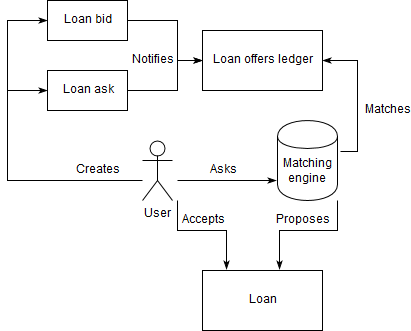
\includegraphics[scale=0.4]{\ImgPath/rys/contracts.png}
\end{center}
	\caption{Loan processing components}
	\label{loan components}
\end{figure}

The next topic that needs explanation is how are the smart contracts structured and how do they interact with the rest of the system. All of this can be seen on the figure \ref{loan components}. The Model consists of three types of smart contracts those are:

\textbf{Preloans}: Depicted in the figure as Loan ask and Loan bid. They are the asks and bids that loan takers and loan givers create, respectively. They contain all of the information enumerated in the specification of a loan as a data object. Ask and bid use the same smart contract as their code, that is Preloan. What differentiates them is what variables are put inside. When two equal Preloans are matched the Preloan being bid deploys the Loan smart contract to the network. All of the parameters are passed from matched Preloans to the final Loan and Loan requires only the information from Preloans to be created. 

\textbf{Ledger}: Depicted in the figure as Loan offers ledger. Ledger is just a smart contract where addresses of created Preloans are stored. It has two columns asks and bids, one for addresses of asks' addresses and the other for bids'. Due to gas costs Ethereum incurs on every stored data and every operation which changes a state, it is of most importance to design such a structure as Ledger in a way that minimises the cost of operations on it and stores only the smallest amount of needed data. The actual implementation of this data structure is explained in the chapter \ref{solidity}. In general most of the operations are left to be done by Java code and thus Ledger's data is mostly read from the Ledger and processed outside. Ledger is not a unique entity. Every user can create his own ledger and then has to supply the ledger address when creating a Preloan. When a Preloan is deployed on the blockchain it calls the ledger whose address it possess and subscribes itself to the Ledger's storage.

\textbf{Loan}: The smart contract that does all of the heavy lifting. After being created from two matched Preloans it transfers the basis to the loan taker, calculates the repayments and starts counting down to the next repayment. All of the repayment and default handling is done exactly as desribed in \textit{Loan processing} process.

\textbf{Matching engine}: As stated many time before, Ethereum consumes gas for every transaction done. That means, such operation as creating a loan will also have to consume funds. Where to get those funds from? There are two solutions. First is, put additional amount of Ether to the Preloan as which will be used to cover transaction costs. The problem is, if gas prices suddenly rise the Preloans will be unusable. The second solution used in this system looks as follows. Every user with an access to the network can query the Ledger for current Preloans, use the matching engine to find matches and than use his own funds to do the transactions. Of course, one immediately sees that this approach has a flaw. Why would anyone bother with paying someone else transactions? The answer is, if you have deployed a Preloan then it is your incentive to commit other transactions as only then will your Preloan will have a chance to take the first place in the queue for being matched. Easy extension using first solution could be used if the whole project was to be developed further. Every creator of a Preloan can assign additional funds to the Preloan which will be than a reward to the person committing the transaction.

The most important architectural decision that has been made here is putting the matching engine outside of the blockchain. It is clearly a security hole. As the matching is done outside of blockchian everyone can do their own matches and then commit them to the network. Of course, one could trace that the transaction should not happen given the Ledger's state but no one will be able to revert it. Nevertheless, one must remember of the gas costs. If the the matching engine was to be put inside blockchain the cost of using it would swing together with the gas prices. Additionally, due to lack of more complex data structures in the Solidity the code would be unsecure and huge meaning even bigger gas costs. Instead the whole matching is accomplished outside of blockchain and the only gas cost related is storing Ledger's data and creating Loan. 

The security issue is still solvable. What has been achieved is not a strong security achieveable by pure blockchain usage but a weak security that still serves it's purpose. All of the contracts have been equipped with validation rules which do not allow for existence of loan whose parameters are harmful to one of the sides. For example it is not possible to match 5\% interest bid with a 3\% interest ask where the final Loan would be 3\% interest rate. Meaning harmful to the loan giver. The word weak means that the Loan achieved are not always the best ones. For example, there is 5\% interst bid and two asks, one has 6\% rate and the other 7\% rate. The best option is match with 7\% ask resulting in a 7\% loan. It is possible for the malicious users to force the 6\% loan meaning not the best possibility. Still the problem evaporates if we add the market forces. If the law of supply and demand where to work properly there would be only one good interest rate and no good and better interest rate. The differences would be simply bought out. In the end, a sacrifice in security has been made for usability.

%-----------------
% Software implementation
%-----------------
\chapter{Software implementation}

Having spent some time on laying out the plans for the software it is now possible to start the construction. The following subchapters will include description of general structure of respective modules. Additionally, more interesting facts about specific technologies backed by code will be presented.

\section{Ethereum network}

Just as there has to be an SQL server if we want to use relational database, there has to be working blockchain network to use blockchain. Generally, the implementation presented here is network-agnostic. That is does not matter whether the network being used is a private network, test network or the main network. All that is needed is an address pointing to Ethereum node server. Further communication with the network is handled by node. The final system has not been tested in a multi-node environment. Partly, due to lack of resources and mainly because working of such network reaches out of the scope of this project. By design of blockchain, communication with a network of one node and a network of many nodes should not differ and thus user of a blockchain should not have to test such scenarios.

\textbf{Geth}, short for GO Ethereum, is an implementation of a Ethereum node in Golang. It is possible to easily start your own network or connect to an existing one using Geth client through command line. Among many Geth includes tools for mining the new hashes or implements the whole web3j RPC standard.  The problem with using Geth is that it's usage is quite low level. Meaning, the user has a lot of command over how the system works but has to do a lot of manual labour. Especially, when doing repetitive tasks such as starting and shutting down the node. Geth is a perfect choice for beginners as it gives a chance to understand every part of the mechanism but at the same time it is unsuitable for development processes being so exhaustive in usage.

\textbf{Ganache} is a tool more suitable for experienced developers willing to omit the standard procedures. The tool is simply a script which automatically handles all of manual labour. By specifying the parameters during start up one can configure his network which is automatically setup with prepared accounts and mining configured as to pass every transaction immediately. Ganache is the tool better suited for software development by hiding a lot of internals of a ethereum node. Which of course could lead to developers unfamiliar with the technology they are using on daily basis. The figure \ref{ganache} presents are working Ethereum node started by Ganache.

\begin{figure}[!htbp]
	\begin{center}
\centering
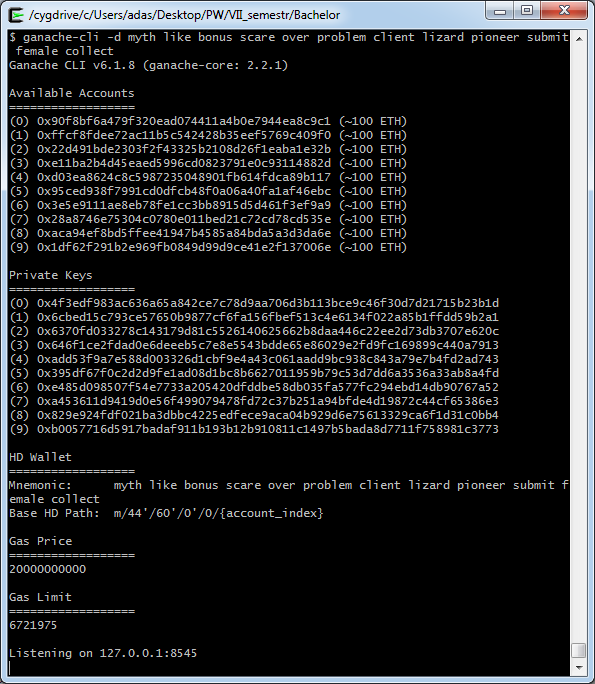
\includegraphics[scale=0.7]{\ImgPath/rys/ganache_cli.png}
\end{center}
	\caption{Ethereum node using Ganache}
	\label{ganache}
\end{figure}



\section{Solidity} \label{solidity}

Solidity is what makes this project different. Being a quite unknown language there are a lot of concepts that have to be explained.

First question anyone may wonder is, how do you compile this? The procedure looks as follows. First, a file with Solidity code has to be created. The file extension for Solidity is .sol. Then an implementation  of a Solidity compiler in arbitrary language has to be used. One can use a JavaScript or Python implementation but for Windows users the easiest way is simply using a compiled binary solc.exe downloadable from Solidity documentation page \cite{solc}. Using compiler on the Solidity file output two files. One binary file and one file with extension .abi. The binary is the actual compiled code. This binary file is later deployed on blockchain, read by EVM and used. The ABI ( Application Binary Interface ) is as the name suggests an interface through which EVM knows the function signatures it will invoke. 

Using solc is a troublesome as using Geth. Fortunately, there have already appeared frameworks who make the development process much faster. The most prominent one and the being used in this project is called \textit{Truffle} \cite{truffle}. Truffle lets you deal with complicated import dependencies by hiding them behind one compile command. It also lets you easily deploy your contracts and interact with them by JavaScript scripts and console. Together Ganache and truffle deal with most of the functionalities of Geth. Ganache provides for the setup environment part and Truffle for the usage of working node part.

Knowing how prepared Solidity ought to be handled we are ready to analyse some actual lines of code.
As an example we will use the Ledger smart contract. The Ledger is used to store addresses of loan asks and loan bids. Taking into account the gas cost of running Solidity code, the data structure has to be written in such a way that will minimise the costs, fulfil the requirements and be secure. The strategy for minimising costs that has been applied here tries to put the minimal amount of code in Solidity and assign as much as possible to Java code. That is why, the addresses are stored in simple unordered arrays. We will sort them using Java. Additionally, the input, read and delete operations are all O(1). Sample code presenting the key concepts can be seen in the listing below.

\begin{lstlisting}
contract Ledger {

 	// Simple array
	address[] public askAddresses;
	address[] public bidAddresses;

	function addAsk(address askAddress) public {
		askAddresses.push(askAddress);
	}

	// Remove element at index and insert the last element there
	function deleteAsk(uint index) public {
		require(index < askAddresses.length);
		if(askAddresses.length > 1){
			askAddresses[index] = askAddresses[askAddresses.length-1];
		}
		delete askAddresses[askAddresses.length-1];
		askAddresses.length--;
	}


	// You have to know index of the element you are looking for
	function getAskAddressAtRow(uint index) constant public returns (address){
		return askAddresses[index];
	}

	function getAskAddressCount() constant public returns (uint){
		return askAddresses.length;
	}

	/* The rest of the code */
}
\end{lstlisting}
 
Fascinating characteristic of Solidity is lack of negative and floating point numbers. Every number here is an unsigned integer 256 bits in length. The decision of creators of Ethereum to dedicate the whole technology to this one number was not ill-minded. Given that Ethereum is serves mostly purely financial needs it is very important to not allow for any rounding errors. Many of modern languages provide two versions of floating point numbers, one for scientific purposes where rounding errors are possible and second, very often called decimal, which assures that up to certain decimal place there will be no rounding errors. Ethereum scraped the whole idea and forced all of Solidity developers to sharpen their math skills and invent ways to do all of their math in integers. The same reasoning removed negative numbers which normally are just a different representation of bits hidden inside a variable.

The whole setup makes non-trivial math functions require non-trivial handling. In this project to calculate repayment of a loan one has to calculate exponential function. Of course, Solidity does not provide an exponential operator as it would allow for floating point numbers. The equation presented in the chapter \ref{loans} has to modified to remove negative exponentials and thus looks as follows.
	
\[C = \frac{(1+r)^n * r * Scale * P}{((1+r)^n - Scale) * Scale}	\]

Where C is monthly installment, r is interest rate per month, P is principal amount/basis, n is a duration of a loan in periods equal to predefined amount of days and Scale is Scale factor which removes fixed point operations. It is very important to not cancel the Scale present in nominator and denominator. If calculated one after another we successfully map the output to integers.

\newpage
The exponential function is computed with the following code.
\begin{lstlisting}
function exp() private constant returns (uint){
	uint s = 0;
	uint N = 1;
	uint B = 1;
	for (uint i = 0; i < precision; ++i){
		s = s.add(scale.mul(N).div(B).div(interestReciprocal**i));
	    N  = N.mul(duration.sub(i));
	    B  = B.mul(i.add(1));
	}
	return s;
}
\end{lstlisting}

The code above computes the formula:
\[	Scale * (1 + \frac{1}{interestReciprocal})^n \]

It does so by using Binomial Theorem, that is the fact that:
\[	(1 + interest) = \sum_{k=0}^n {n \choose k} interest^k \]

The loop above computes first k values of the sum. The variable k is depicted in the loop as precision. The approximation works because every next element in the sum is smaller by considerably amount and thus even precision equal to eight grants sufficient quality of approximation. The general experience shows, that what constitutes a simple operator invocation in even low level languages, here requires math savviness.

The last element of Solidity that is worth mentioning are the tests. As stated many times throughout this paper Solidity is a fragile language, meaning that it is easy to make mistakes and the mistakes could be very costly. It is obligatory then to maximize test coverage. Moreover, it also helps for future development. For example, in the case of this project. If some Java code invoking Solidity returns error we have two possible sources of error. Either the solidity code is broken or the data we input is incorrect. Testing Solidity allows us to erode the first possibility and find the error much quicker saving a lot of our precious time. 

How does one write tests for Solidity? With help comes once again the Truffle framework. Besides compilation or deployment it also provides testing framework. It is possible to write high level tests using JavaScript or low level ones using Solidity itself. In this project all of tests have been written in JavaScript as none of the cases required more low level handling. The Truffle extends a widely used JavaScript testing framework Mocha which uses asynchronous capabilities of JavaScript to write very clean test cases. An example test case can be seen in the listing below. As a proof of the work done for this project and it's correctness a test suite is presented in the figure \ref{tests}

\begin{lstlisting}
contract('Ledger unit test', function(accounts){
  it("should allow to remove ask addresses", function() {
    return Ledger.deployed().then(function(instance){
      ledger = instance;
      return ledger.deleteAsk(0);
    }).then(function() {
      return ledger.getAskAddressCount();
    }).then(function(addressesLength) {
      assert.equal(addressesLength, 2, "Addresses length after delete is " + addressesLength + " instead of 2");
    });
  });
}
\end{lstlisting}

\begin{figure}[!htbp]
	\begin{center}
\centering
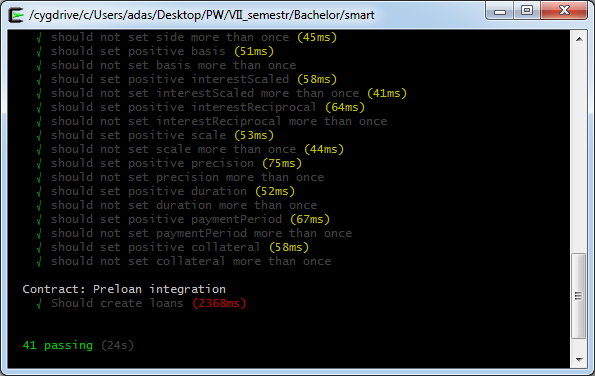
\includegraphics[scale=0.7]{\ImgPath/rys/test_pass.png}
\end{center}
	\caption{Successful test suite run}
	\label{tests}
\end{figure}

\newpage

\section{Java}

All of Exchange Engine and GUI components are written in Java. Being one of the most known languages in the world there will no remarks over the language itself. What this subchapter will concern are mostly the classes, their dependencies and the structures employed in the project.

\begin{figure}[!htbp]
	\begin{center}
\centering
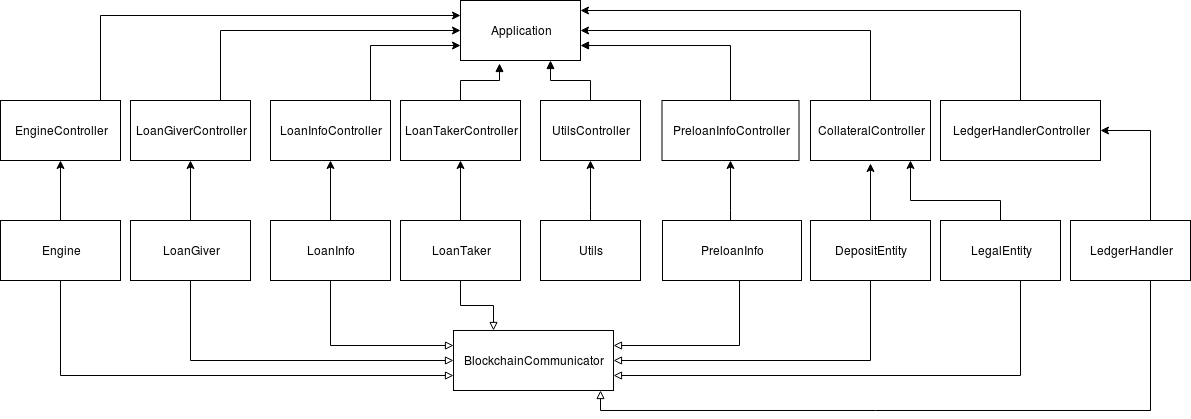
\includegraphics[scale=0.4]{\ImgPath/rys/exchange_class.png}
\end{center}
	\caption{Simplified class diagram of the exchange engine}
	\label{engine class}
\end{figure}

We start of with the class diagram of the Exchange component, that is figure \ref{engine class} . The whole component is a stand-alone application that starts a server servicing REST requests. For this purpose a Spring Boot framework has been employed. As such, the architecture seen above is mostly a pattern of using this framework. The diagram is simplified as it doesn't present Data Transport Objects(DTO) which are not important in an functional overview.

The respective components serve following purposes:

\textbf{Application} - is the JVM start point. It contains the \textit{main} function and starts automatically the server. All of the configurations are already supplied by Spring Boot. As a result, developer does not have to waste time on this aspect and can focus on the aim of the project. 

Moreover, the Application class is coupled with a Swagger class and thus creates Swagger's pages out of the box. Swagger is a documentation library which automatically searches for all the REST end-points defined in the application and presents them in a compact and user friendly form. It is also possible to use Swagger for sending the REST requests making the debuggin process much faster. The traditional way of using debugging REST endpoints would be through usage of curl in command line, which was a troublesome and mistake ridden process.

\textbf{Controller} - all of the classes which end with a Controller word contain the actual information about what REST end-points are presented by the application. Every Controller encapsulates one domain of functionalities and can be easily replaced or detaches without affecting the whole structure. For example, the LoanInfoController defines end-points allowing for access to information of a deployed loan. The Controllers do not implement the functions themselves, they only present interfaces to the outside world and direct the requests to respective entity classes. After, the computations are done a Controller receives the results and sends them back to the inquirer. 

The Controllers are not connected with the Application class by hardcoded classes references. Technique called dependency injection is used here. Upon launching the application The Spring Boot framework looks for classes annotated with keyword \textit{@RestController}, then inside those classes it looks for functions annotated with keyword \textit{@PostMapping} or \textit{@GetMapping}, this annotation specifies also the path which has to be put into URL to access the function and what parameters ought to be supplied. Finally, the paths and their respective classes are processed into the server and are able to be used by users.

\textbf{Entity} - the second layer presented in the diagram consists of classes which do the actual hard work. Those classes are instantiated by Controller classes and asked for fetching data or completing some kind of computations. For example, the Engine class receives an address of a Ledger, fetches the Ledger data from blockchain and matches the bids and asks so that proper Loans can be created. Different set of tasks is done by the Utils class which for example allows to encrypt information using RSA or ASE keys.

\textbf{Blockchain Communicator} - is a class inherited by all of the Entity classes which have to communicate with the blockchain. The communicator provides ready functions which use the Web3j library to ,for example, connect with the blockchain or load some contracts. The library communicates with blockchain in an asynchronous manner. For this purpose Completable Futures are used, an invention brought into life with Java 8.

\begin{figure}[!htbp]
	\begin{center}
\centering
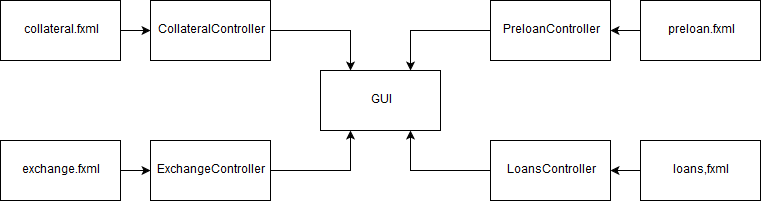
\includegraphics[scale=0.4]{\ImgPath/rys/gui_class.png}
\end{center}
	\caption{Simplified class diagram of the gui application}
	\label{gui class}
\end{figure}

The next application written in Java is the GUI component of which class diagram we see on figure \ref{gui class} . Just as the Engine, the whole component is a stand-alone application. It uses built-in Java library called JavaFX, which allows for creation of modern desktop applications. The blocks in the diagram represent the following classes:

\textbf{GUI} - in the exact same manner as for the Spring Boot application we need a starting class, whose only purpose is to place a main function and define starting configurations. That is in this example the first window to open. JavaFX based it's core on multi-threading. The thread which starts the actual GUI branches out from the thread which starts the Java program.

\textbf{Controller} - is Java class which is supposed to be assigned to an fxml file. The Java class can handle events coming from the fxml files. It can manipulate the windows and values inside windows. JavaFX provides automatic dependency injection for window components inside Controller classes. So that it is only required to define a variable whose name is the same as an ID of a window component and the references will be automatically injected. Removing the need for any type of searching for window components. Controller is also the class which send the REST requests to the Engine component. For this, Task objects provided by JavaFX are used. The Tasks have to given certain attributes and callback functions. When started they create their own thread where they handle the network I/O. This way, User Experience is not obstructed with lags.

\textbf{fxml files} - could be compared to HTML files. They use XML to define the structure of a window. CSS files are attached to them to define styles. Finally, each fxml has a controller assigned to it. Every component of the window can assigned some event and the event handler in the controller. The fxml files express great modularity capabilities. They can include other fxml files, which have their own controller. For example, every main window includes a navBar.fxml which handles switches between windows. This way a lot of redundancy can be avoided. In general, the material design rules were tried to be followed as to make the GUI as aesthetically pleasing as possible.

\section{Summary}

In this section screenshots of the GUI are presented. The images will only present general form of the windows and not all of the functionalities will be seen as the GUI serves only a supporting role in this project.


\chapter{Usage showcase}

The last chapter is dedicated towards a showcase of a typical use of the system. The presentation should serve as a proof of the work done and a source of admiration for blockchain. 

\begin{enumerate}
\item Start the ethereum node, matching engine and application GUI.
\item Create a ledger \ref{create ledger}.

\begin{figure}[!htbp]
	\begin{center}
\centering
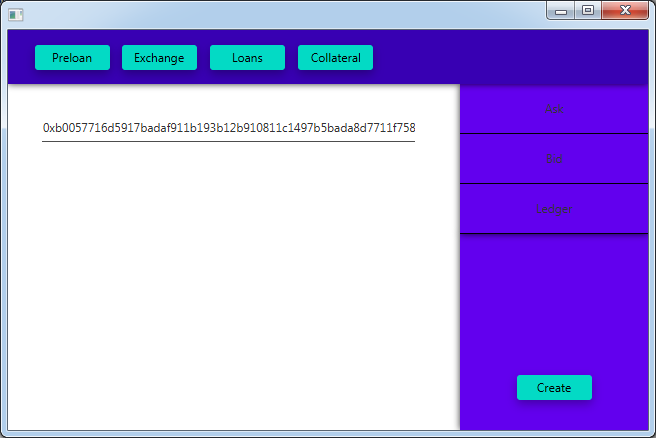
\includegraphics[scale=0.4]{\ImgPath/rys/create_ledger.png}
\end{center}
	\caption{Ledger creator}
	\label{create ledger}
\end{figure}

\item Create deposit \ref{create deposit}.

\begin{figure}[!htbp]
	\begin{center}
\centering
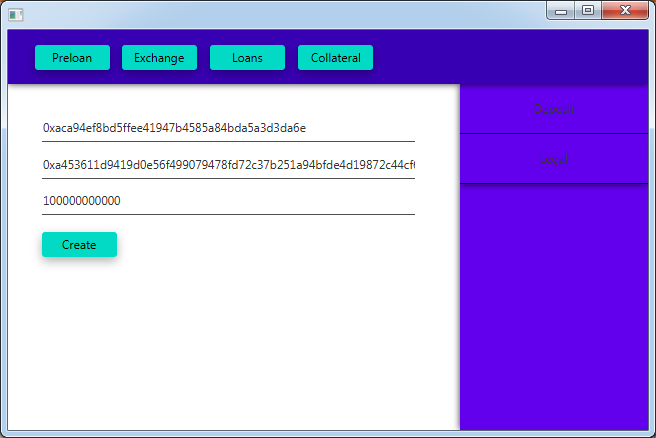
\includegraphics[scale=0.4]{\ImgPath/rys/create_deposit.png}
\end{center}
	\caption{Deposit creator}
	\label{create deposit}
\end{figure}

\item Create Preloans, bid and ask \ref{create bid}.

\begin{figure}[!htbp]
	\begin{center}
\centering
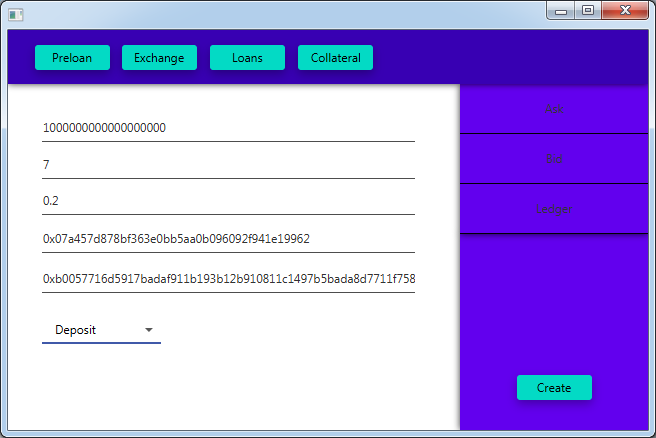
\includegraphics[scale=0.4]{\ImgPath/rys/create_bid.png}
\end{center}
	\caption{Bid creator}
	\label{create bid}
\end{figure}

\item See if the Preloans appear on the exchange \ref{check exchange}.

\begin{figure}[!htbp]
	\begin{center}
\centering
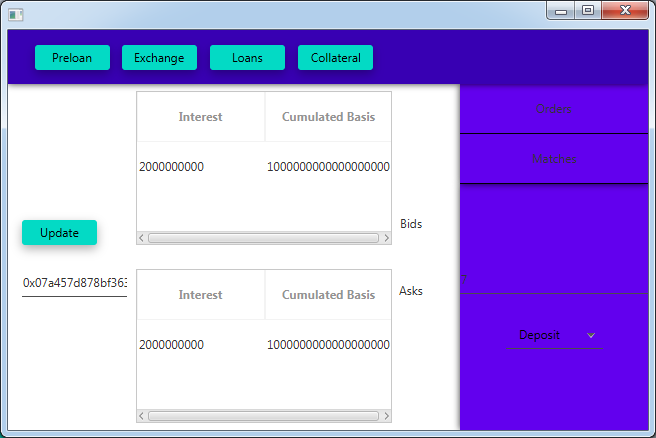
\includegraphics[scale=0.4]{\ImgPath/rys/check_exchange.png}
\end{center}
	\caption{Exchange with created Preloans}
	\label{check exchange}
\end{figure}

\item Match Preloans and create a Loan \ref{check loans}.

\begin{figure}[!htbp]
	\begin{center}
\centering
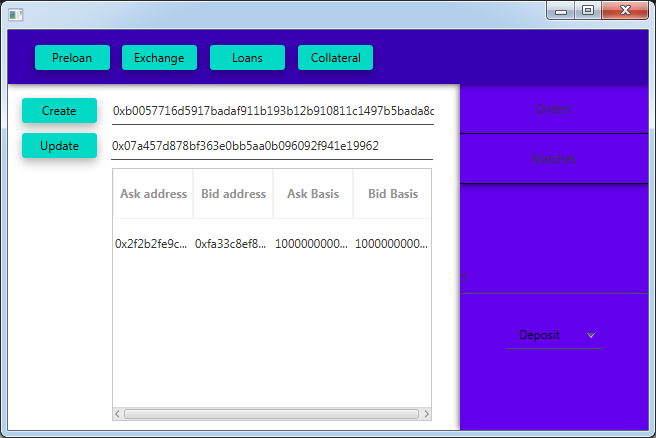
\includegraphics[scale=0.4]{\ImgPath/rys/check_loans.png}
\end{center}
	\caption{Matched Preloans}
	\label{check loans}
\end{figure}

\item Check the parameters of a created Loan \ref{check loan}.

\begin{figure}[!htbp]
	\begin{center}
\centering
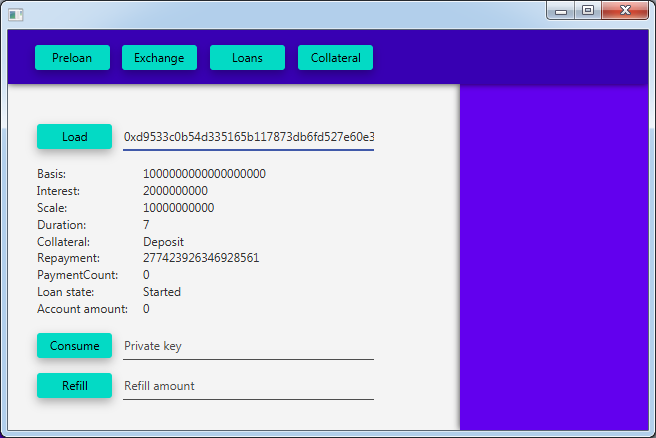
\includegraphics[scale=0.4]{\ImgPath/rys/check_loan.png}
\end{center}
	\caption{Loan parameters}
	\label{check loan}
\end{figure}

\item Refill the loan and then consume the refill \ref{check consume}.

\begin{figure}[!htbp]
	\begin{center}
\centering
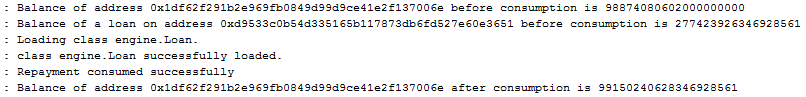
\includegraphics[scale=0.7]{\ImgPath/rys/check_consume.png}
\end{center}
	\caption{Logs of a loan consumption process}
	\label{check consume}
\end{figure}

\item Consume without a refill and receive funds from deposit \ref{check deposit}.

\begin{figure}[!htbp]
	\begin{center}
\centering
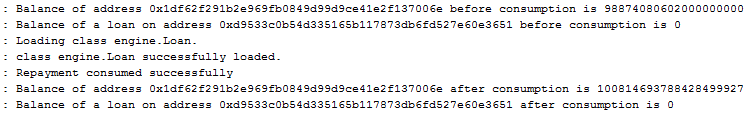
\includegraphics[scale=0.7]{\ImgPath/rys/check_deposit.png}
\end{center}
	\caption{Logs of funds recovery process using deposit}
	\label{check deposit}
\end{figure}

\end{enumerate}


\begin{thebibliography}{99}
\addcontentsline{toc}{chapter}{Bibliography}
\bibitem{Bitcoin}{Satoshi Nakamoto , Access date: 02.10.2018 , ,,Bitcoin: A Peer-to-Peer Electronic Cash System'', \url{https://bitcoin.org/bitcoin.pdf}}
\bibitem{Venezuela}{Simon Chandler, Access date: 02.10.2018, ,,How Venezuela Came to Be One of the Biggest Markets for Crypto in the World'', \url{https://goo.gl/s1t7nm}}
\bibitem{Silkroad}{Silk Road Drugs, Access date: 02.10.2018, ,,The Effect Of Silk Road On Bitcoin And Tor'', \url{https://silkroaddrugs.org/the-effect-of-silk-road-on-bitcoin-and-tor/}}
\bibitem{Bitcoinwiki}{Access date: 02.10.2018, \url{https://en.bitcoin.it/wiki/Difficulty}}
\bibitem{Ethereum}{Access date: 02.10.2018, \url{https://github.com/ethereum/wiki/wiki/White-Paper}}
\bibitem{energy}{Access date: 02.10.2018, \url{https://digiconomist.net/bitcoin-energy-consumption}}
\bibitem{dapps}{Access date: 02.10.2018, \url{https://www.stateofthedapps.com/}}
\bibitem{tokens}{Access date: 02.10.2018, \url{https://etherscan.io/tokens}}
\bibitem{ethyellow}{Gavin Wood, Access date: 02.10.2018, \url{https://gavwood.com/paper.pdf}}
\bibitem{gas}{Access date: 02.10.2018, \url{https://github.com/djrtwo/evm-opcode-gas-costs}}
\bibitem{secure}{Access date: 02.10.2018, \url{https://solidity.readthedocs.io/en/v0.4.24/security-considerations.html}}
\bibitem{RPC}{Access date: 02.10.2018, \url{https://github.com/ethereum/wiki/wiki/JSON-RPC}}
\bibitem{ethlend}{Access date: 03.10.2018, \url{https://ethlend.io/#/main}}
\bibitem{btcpop}{Access date: 04.10.2018, \url{https://btcpop.co/}}
\bibitem{bitbond}{Access date: 04.10.2018, \url{https://www.bitbond.com/}}
\bibitem{credible}{Access date: 04.10.2018, \url{https://crediblefriends.com/}}
\bibitem{kambo}{Access date: 04.10.2018, \url{https://www.kambo.io/}}
\bibitem{unchained}{Access date: 04.10.2018, \url{https://www.unchained-capital.com/}}
\bibitem{makerdao}{Access date: 04.10.2018, \url{https://makerdao.com/}}
\bibitem{othera}{Access date: 04.10.2018, \url{https://www.othera.io/}}
\bibitem{othera}{Google, Access date: 09.10.2018, \url{https://material.io/design/}}
\bibitem{solc}{Access date: 09.10.2018, \url{https://solidity.readthedocs.io/en/v0.4.21/installing-solidity.html}}
\bibitem{truffle}{Access date: 09.10.2018, \url{https://truffleframework.com/}}


\end{thebibliography}

\zakonczenie  % wklejenie recenzji i opinii

\end{document}
%+++ END +++
